In epistemology ranking theory is a theory of belief and its revision. It studies how an ideal doxastic agent should organize her beliefs and conditional beliefs at a given moment in time, and how she should revise her beliefs and conditional beliefs across time when she receives new information. In this entry I will first present some background, most notably the AGM theory of belief revision \citep{agm85}. In order to motivate the introduction of ranking theory I will then focus on the problem of \emph{iterated} belief revisions. After presenting the elements of ranking theory \citep{s88, s12} I will show how this theory solves the problem of iterated belief revisions. I will conclude by sketching two areas of future research and by mentioning applications of ranking theory outside epistemology. Along the way we will see how ranking theory, a theory of belief, compares to subjective probability theory or Bayesianism, which is a theory of partial beliefs or degrees of belief.


\section{Introduction}

Sophia believes many things, among others that it will rain on Tuesday, that it will be sunny on Wednesday, and that weather forecasts are always right. Belief revision theory tells Sophia how to revise her beliefs when she learns %on Monday
that the weather forecast for Tuesday and Wednesday predicts rain. As we will see, this depends on the details of her beliefs, but under one way of filling in the details she should keep her belief that it will rain on Tuesday and give up her belief that it will be sunny on Wednesday. To state in full detail how Sophia should revise her beliefs when she learns new information we need a representation of her old beliefs and of the new information she receives.

In this entry I will focus on ideal doxastic agents who do not suffer from the computational and other physical limitations of ordinary doxastic agents such as people and computer programs. These ideal doxastic agents get to voluntarily decide what to believe (and to what degree of numerical precision); they never forget any of their (degrees of) beliefs; and they always believe all logical and conceptual truths (to a maximal degree). We may perhaps define a (doxastic or cognitive) agent to be \emph{ideal} just in case any (cognitive) action that is physically possible is an action that is possible for her. Such ideal agents ought to do exactly that which they ought to do if they could, where the `can' that is hidden in the `could' expresses possibility for the agent, not metaphysical possibility. Hence the principle that \emph{Ought Implies Can} does not put any constraints on what an ideal agent should do, and on what an ideal doxastic agent should believe.

Belief revision theory models belief as a qualitative attitude towards sentences or propositions: the ideal doxastic agent believes a proposition, or she disbelieves the proposition by believing its negation, or she suspends judgment with respect to the proposition and its negation. This is different from the theory of subjective probabilities, also known as \emph{Bayesianism} (\citealt{e11, e11b}; Titelbaum, \citethisvolume{thisvolume:titelbaum}; \citealt{w11}; Wenmackers, \citethisvolume{thisvolume:wenmackers}), where belief is modeled as a quantitative attitude towards a proposition: the ideal doxastic agent believes a proposition to a specific degree, her degree of belief, or credence, for the proposition. However, we will see that, in order to adequately model conditional beliefs and iterated belief revisions, ranking theory also models the ideal agent's doxastic state with numbers, and thus more than just the set of propositions she believes. Genin (\citethisvolume{thisvolume:genin}) discusses the relation between belief and degree of belief.

\section{Belief Revision}

\citet{s88,s90} develops ranking theory in order to fix a problem that besets the AGM theory of belief revision. In order to provide some background for ranking theory I will first present the AGM theory. Ranking theory will then arise naturally out of the AGM theory. The latter theory derives its name from the seminal paper by \citet{agm85}. Comprehensive overviews can be found in \citet{g88b}, \citet{gr95}, \citet{r01}, and Lin (\citethisvolume{thisvolume:lin}).

One version of the AGM theory of belief revision represents the ideal doxastic agent's old beliefs, her doxastic state at a given moment in time, by a set of sentences from some formal language, her \emph{belief set}, together with an \emph{entrenchment ordering} over these sentences. The entrenchment ordering represents how firmly the ideal doxastic agent holds the beliefs in her belief set. It represents the details of the ideal agent's doxastic state. The new information is represented by a single sentence. The AGM theory distinguishes between the easy case, called \emph{expansion}, and the general case, called \emph{revision}. In expansion the new information does not contradict the ideal doxastic agent's old belief set and is simply added. In revision the new information may contradict the ideal doxastic agent's old belief set. The general case of revision is difficult, because the ideal doxastic agent has to turn her old belief set, which is assumed to be consistent, into a new belief set that contains the new information and is consistent. Usually the general case is dealt with in two steps. In a first step, called \emph{contraction}, the old belief set is cleared of everything that contradicts the new information. In a second step one simply expands by adding the new information. This means that the difficult doxastic task is handled by contraction, which turns the general case of revision into the easy case of expansion.

A formal language $\cal L$ is defined inductively, or recursively, as follows. $\cal L$ contains the contradictory sentence $\ulcorner\bot\urcorner$ and all elements of a countable set of propositional variables $PV=\left\{\ulcorner P\urcorner,\ulcorner Q\urcorner,\ulcorner R\urcorner,\ldots\right\}$. Furthermore, whenever $A$ and $B$ are sentences of $\cal L$, then so are the negations of $A$ and of $B$, $\ulcorner\neg A\urcorner$ and $\ulcorner\neg B\urcorner$, respectively, as well as the conjunction of $A$ and $B$, $\ulcorner\left(A\wedge B\right)\urcorner$. Finally, nothing else is a sentence of $\cal L$. The new information is represented by a single sentence $A$ from $\cal L$. The ideal agent's doxastic state is represented by a set of sentences, her belief set $\cal B\subseteq L$, plus an entrenchment ordering $\preceq$ for $\cal B$. The entrenchment ordering, which represents the details of the ideal doxastic agent's beliefs, orders the agent's beliefs according to how reluctant she is to give them up: the more entrenched a belief, the more reluctant she is to give it up.

The entrenchment ordering does most of the work in a revision of the agent's beliefs. Suppose the agent receives new information that contradicts her belief set. Since the new belief set that results from the revision has to be consistent, some of the old beliefs have to go. The entrenchment ordering determines which beliefs have to go first: the least entrenched beliefs are the beliefs that have to go first. If giving up those is not enough to restore consistency, the beliefs that are next in the entrenchment ordering have to go next. And so on. The beliefs that would be given up last are the most entrenched ones. According to Maximality, they are the tautological sentences, which are always believed and never given up, because doing so cannot restore consistency. On the other end of the spectrum are the least entrenched sentences. According to Minimality, they are the sentences the agent does not even believe to begin with. These sentences do not belong to the agent's belief set and so are gone before the revision process has even begun.

If one sentence logically implies another sentence, then, according to Dominance, the latter cannot be more entrenched than the former, as giving up the belief in the latter sentence is to also give up the belief in the former sentence. Dominance implies that the entrenchment ordering is \emph{reflexive}: every sentence is at least as entrenched as itself. According to Conjunctivity, two sentences cannot both be more entrenched than their conjunction: one cannot give up one's belief in a conjunction without giving up one's belief in at least one of the conjuncts. In combination with Dominance, Conjunctivity implies that the entrenchment ordering is \emph{connected}: any two sentences can be compared to each other in terms of their comparative entrenchment. That is, either the first sentence is at least as entrenched as the second sentence, or the second sentence is at least as entrenched as the first sentence, or both. Finally, to ensure that the entrenchment ordering is a well-behaved ordering relation, it is assumed to be \emph{transitive} by Transitivity.

More precisely, where $\vdash$ is the logical consequence relationship on $\cal L$ and $Cn\left(\cal B\right)=\left\{A\in\begin{cal}L\end{cal}:\begin{cal}B\end{cal}\vdash A\right\}$ is the set of logical consequences of $\cal B$ (and $\emptyset$ is the empty set $\left\{\right\}$), the entrenchment ordering has to satisfy the following postulates. For all sentences $A$, $B$, and $C$ from $\cal L$:
\begin{enumerate}
\item[$\preceq$1.] If $A\preceq B$ and $B\preceq C$, then $A\preceq C$.\hfill Transitivity
\item[$\preceq$2.] If $\left\{A\right\}\vdash B$, then $A\preceq B$.\hfill Dominance
\item[$\preceq$3.] $A\preceq A\wedge B$ or $B\preceq A\wedge B$.\hfill Conjunctivity
\item[$\preceq$4.] Suppose $\begin{cal}B\end{cal}\not\vdash\bot$. Then $A\notin\cal B$ if, and only if,\\$\phantom{M}$\hspace{1em} for all $B\in\cal L$: $A\preceq B$.\hfill Minimality
\item[$\preceq$5.] If $A\preceq B$ for all $A\in\cal L$, then $\emptyset\vdash B$.\hfill Maximality
\end{enumerate}

The work that is done by the entrenchment ordering in a revision of the agent's beliefs can also be described differently in terms of expansion, revision, and contraction, which turn belief sets and new information into belief sets (see Caie, \citethisvolume{thisvolume:caie}). Formally they are functions from $\powerset\!\left(\cal L\right)\times\cal L$ into $\powerset\!\left(\cal L\right)$.

Expansion $\dot+$ turns each old belief set $\cal B\subseteq L$ and each sentence $A$ from $\cal L$ into a new belief set $\begin{cal}B\end{cal}\dot+A=Cn\left(\begin{cal}B\end{cal}\cup\left\{A\right\}\right)$. This is the easy case described earlier about which there is little more to be said.

The difficult and more interesting case is revision $*$, which turns each old belief set $\cal B\subseteq L$ and each sentence $A$ from $\cal L$ into a new belief set $\begin{cal}B\end{cal}*A$. The operator $*$ is required to satisfy a number of postulates.

Closure requires revised belief sets to be closed under the logical consequence relation: after the revision is completed, the agent ought to believe all (and only) the logical consequences of the revised belief set. Congruence is similar in spirit to Closure and requires that it is the content of the new information received, and not its particular formulation, that determines what is added, and what is removed, from the agent's belief set in a revision. Success requires that revising a belief set by new information succeeds in adding the new information to the agent's belief set---and, given Closure, all sentences it logically implies. Consistency requires the revised belief set to be consistent as long as the new information is consistent. The remaining postulates all formulate different aspects of the idea that, when revising her belief set by new information, the agent should add and remove as few beliefs as possible from her belief set, subject to the constraints that the resulting belief set is consistent and that the new information has been added successfully.

Inclusion requires that revising a belief set does not create any new beliefs that are not also created by simply adding the new information. In a sense it says that expansion is a special case of revision.
Preservation requires that revising a belief set by new information that does not contradict the agent's old belief set does not lead to the loss of any beliefs.  %It can be formulated as the requirement that, in contracting by a given sentence, only those beliefs get removed from the belief set that get removed in all contractions by any sentence that is logically equivalent to the original one.
%Recovery requires that contracting a belief set by a sentence removes as few beliefs as possible so that adding the removed sentence again afterwards allows the agent to recover all her previously removed beliefs.
Conjunction 1 requires that, when revising her belief set by a conjunction, the agent adds \emph{only} beliefs that she also adds when first revising her belief set by one of the two conjuncts, and then adding the second conjunct. Conjunction 2 requires that, when revising her belief set by a conjunction, the agent adds \emph{all} beliefs that she adds when first revising her belief set by one of the two conjuncts, and then adding the second conjunct---provided the second conjunct is consistent with the result of revising her belief set by the first conjunct. More precisely, a revision function has to satisfy the following postulates. For all sets of sentences $\cal B\subseteq L$ and all sentences $A$ and $B$ from $\cal L$:
\begin{enumerate}
\item[$*$1.] $\begin{cal}B\end{cal}*A=Cn\left(\begin{cal}B\end{cal}*A\right)$.\hfill Closure
\item[$*$2.] $A\in\begin{cal}B\end{cal}*A$.\hfill Success
\item[$*$3.] $\begin{cal}B\end{cal}*A\subseteq Cn\left(\begin{cal}B\end{cal}\cup\left\{A\right\}\right)$.\hfill Inclusion
\item[$*$4.] If $\begin{cal}B\end{cal}\not\vdash\neg A$, then $\begin{cal}B\end{cal}\subseteq\begin{cal}B\end{cal}*A$.\hfill Preservation
\item[$*$5.] If $\left\{A\right\}\vdash B$ and $\left\{B\right\}\vdash A$, then $\begin{cal}B\end{cal}*A=\begin{cal}B\end{cal}*B$.\hfill Congruence
\item[$*$6.] If $\emptyset\not\vdash\neg A$, then $\bot\not\in\begin{cal}B\end{cal}*A$.\hfill Consistency
\item[$*$7.] $\begin{cal}B\end{cal}*\left(A\wedge  B\right)\subseteq Cn\left(\left(\begin{cal}B\end{cal}*A\right)\cup\left\{B\right\}\right)$.\hfill Conjunction 1
\item[$*$8.] If $\neg B\not\in\begin{cal}B\end{cal}*A$, then\\$\phantom{M}$\hspace{1em}  $Cn\left(\left(\begin{cal}B\end{cal}*A\right)\cup\left\{B\right\}\right)\subseteq\begin{cal}B\end{cal}*\left(A\wedge B\right)$.\hfill Conjunction 2
\end{enumerate}

The two-step view of revision described previously is known as the \emph{Levi identity} \citep{l77}. It has the ideal doxastic agent first contract $\dotminus$ her old belief set $\cal B$ by the negation of the new information, $\neg A$, thus making it consistent with the new information (as well as everything logically implied by the new information). Then it has her expand the result $\begin{cal}B\end{cal}\dotminus\neg A$ by adding the new information $A$:
$$\begin{cal}B\end{cal}*A=Cn\left(\left(\begin{cal}B\end{cal}\dotminus\neg A\right)\cup\left\{A\right\}\right).$$
The Levi identity puts contraction center stage in the revision process. Contraction $\dotminus$ turns each old belief set $\cal B\subseteq L$ and each sentence $A$ from $\cal L$ into a ``reduced'' belief set $\begin{cal}B\end{cal}\dotminus A$ that is cleared of $A$ as well as everything logically implying $A$. It is required to satisfy the following postulates%, which result from postulates $*1$-$*8$ for revision and the Levi identity, and thus have the same motivation as $*1$-$*8$ and $\preceq 1$-$\preceq 5$
. For all sets of sentences $\cal B\subseteq L$ and all sentences $A$ and $B$ from $\cal L$:
\begin{enumerate}
\item[$\dotminus$1.] $\begin{cal}B\end{cal}\dotminus A=Cn\left(\begin{cal}B\end{cal}\dotminus A\right)$.\hfill Closure
\item[$\dotminus$2.] If $\emptyset\not\vdash A$, then $A\not\in Cn\left(\begin{cal}B\end{cal}\dotminus A\right)$.\hfill Success
\item[$\dotminus$3.] $\begin{cal}B\end{cal}\dotminus A\subseteq Cn\left(\cal B\right)$.\hfill Inclusion
\item[$\dotminus$4.] If $\begin{cal}B\end{cal}\not\vdash A$, then $\begin{cal}B\end{cal}\dotminus A=\cal B$.\hfill Vacuity
\item[$\dotminus$5.] If $\left\{A\right\}\vdash B$ and $\left\{B\right\}\vdash A$, then $\begin{cal}B\end{cal}\dotminus A=\begin{cal}B\end{cal}\dotminus B$.\hfill Congruence
\item[$\dotminus$6.] $Cn\left(\begin{cal}B\end{cal}\right)\subseteq Cn\left(\left(\begin{cal}B\end{cal}\dotminus A\right)\cup\left\{A\right\}\right)$.\hfill Recovery
\item[$\dotminus$7.] $\left(\begin{cal}B\end{cal}\dotminus A\right)\cap\left(\begin{cal}B\end{cal}\dotminus B\right)\subseteq\begin{cal}B\end{cal}\dotminus \left(A\wedge B\right)$.\hfill Conjunction 1
\item[$\dotminus$8.] If $A\not\in\begin{cal}B\end{cal}\dotminus \left(A\wedge B\right)$, then $\begin{cal}B\end{cal}\dotminus \left(A\wedge B\right)\subseteq\begin{cal}B\end{cal}\dotminus A$.\hfill Conjunction 2
\end{enumerate}
Closure requires contracted belief sets to be closed under the logical consequence relation: after the contraction is completed, the agent ought to believe all (and only) the logical consequences of the contracted belief set. Congruence is similar in spirit to Closure and requires that it is the content of the sentence to be removed, and not its particular formulation, that determines what is removed from the agent's belief set in a contraction. Success requires that contracting a belief set by a sentence that is not tautological succeeds in removing this sentence from a belief set---and, given Closure, all sentences logically implying it. Inclusion requires that contracting a belief set does not add any beliefs to the belief set. The remaining postulates all formulate different aspects of the idea that, when contracting her belief set by a sentence, the agent should remove as few beliefs as possible from her belief set, subject to the constraints that the resulting belief set is consistent and that the sentence to be removed, together with all sentences logically implying it, is removed successfully.

Vacuity requires that contracting a belief set by a sentence leaves the belief set unchanged if the sentence that was to be removed was not even part of the belief set to begin with. %It can be formulated as the requirement that, in contracting by a given sentence, only those beliefs get removed from the belief set that get removed in all contractions by any sentence that is logically equivalent to the original one.
Recovery requires that contracting a belief set by a sentence removes as few beliefs as possible so that adding the removed sentence again afterwards allows the agent to recover all her previously removed beliefs. Conjunction 1 requires that, when contracting her belief set by a conjunction, the agent does not remove any beliefs that she does not also remove when contracting by one or the other of the two conjuncts alone. Finally, Conjunction 2 requires the following: if a conjunct is removed in contracting a belief set by a conjunction, then no belief gets removed in contracting the belief set by this conjunct that does not also get removed in contracting this belief set by the entire conjunction. The idea behind the last two postulates is that giving up one of its conjuncts is all the ideal doxastic agent needs to do in order to give up an entire conjunction.

The Levi identity turns each contraction operator $\dotminus$ satisfying $\dotminus 1$\,--\,$\dotminus 8$ into a revision operator $*$ satisfying $*1$\,--\,$*8$. The converse is true of the \emph{Harper identity} \citep{h76a}. The latter has the ideal doxastic agent first revise the old belief set $\cal B$ by the negation of the new information, $\neg A$. Then it has her remove everything from the result $\begin{cal}B\end{cal}*\neg A$ that was not already also a logical consequence of the old belief set $\cal B$:
$$\begin{cal}B\end{cal}\dotminus A=\left(\begin{cal}B\end{cal}*\neg A\right)\cap Cn\left(\cal B\right).$$
If we have a belief set $\cal B\subseteq L$ we can use an entrenchment ordering $\preceq$ for $\cal B$ to define a revision operator $*$ for $\cal L$ as follows. For every sentence $A$ from $\cal L$:
$$\begin{cal}B\end{cal}*A=Cn\left(\left\{B\in\begin{cal}L\end{cal}:\neg A\prec B\right\}\cup\left\{A\right\}\right),$$
where $A\prec B$ holds if, and only if, $A\preceq B$ and $B\not\preceq A$.

The idea behind this equation is the following. When the ideal doxastic agent revises $*$ her old belief set $\cal B$ by the new information $A$ she first has to clear $\cal B$ of $\neg A$ as well as everything else that is as entrenched as, or less entrenched than, $\neg A$. For instance, $\cal B$ also has to be cleared of everything that logically implies $\neg A$. However, it follows from the definition of an entrenchment ordering that all sentences $B$ from the ideal doxastic agent's old belief set $\cal B$ that are more entrenched than $\neg A$ can be preserved. This gives us the ``preserved'' belief set $\left\{B\in\begin{cal}L\end{cal}:\neg A\prec B\right\}$. Then the ideal doxastic agent adds the new information $A$ to obtain $\left\{B\in\begin{cal}L\end{cal}:\neg A\prec B\right\}\cup\left\{A\right\}$. Finally she adds all sentences that are logically implied by the preserved belief set together with the new information. As shown by \citet{g88b} and \citet{gm88} one can then prove
\begin{theorem}\label{th1}
Let $\cal L$ be a formal language. For each set of sentences $\cal B\subseteq L$ and each entrenchment ordering $\preceq$ for $\cal B$ satisfying $\preceq \!\! 1$\,--\,$\preceq \!\! 5$ there is a revision operator $*$ from $\left\{\cal B\right\}\times\cal L$ into $\powerset\left(\cal L\right)$ satisfying $*1$\,--\,$*8$ restricted to $\cal B$ such that for all $A\in\cal L$:
$$\begin{cal}B\end{cal}*A=Cn\left(\left\{B\in\begin{cal}L\end{cal}:\neg A\prec B\right\}\cup\left\{A\right\}\right).$$
For each revision operator $*$ from $\powerset\left(\cal L\right)\times\cal L$ into $\powerset\left(\cal L\right)$ satisfying $*1$\,--\,$*8$ and each set of sentences $\cal B\subseteq L$ there is an entrenchment ordering $\preceq$ for $\cal B$ satisfying $\preceq \! 1$\,--\,$\preceq \! 5$ such that for all $A\in\cal L$:
$$\begin{cal}B\end{cal}*A=Cn\left(\left\{B\in\begin{cal}L\end{cal}:\neg A\prec B\right\}\cup\left\{A\right\}\right).$$
\end{theorem}
This theorem states that the postulates for entrenchment orderings translate into the postulates for revision functions, and conversely. Caie (\citethisvolume{thisvolume:caie}, Section 2.3) states the analogous theorem regarding the relationship between the postulates for entrenchment orderings and the postulates for contraction functions.

There is a different way of representing postulates $*1$\,--\,$*8$ for revision operators $*$ due to \citet{g88}. Similar to Lewis' (\citeyear{l73}) theory of counterfactuals it uses systems of spheres defined on a set of possible worlds instead of entrenchment orderings defined on a formal language (for more on counterfactuals see Briggs, \citethisvolume{thisvolume:briggs}). A set of possible worlds can be thought of as a set of complete, or maximally specific, descriptions of the way the world could be. One approach, used by \citet{g88}, is to identify possible worlds with maximally consistent sets of sentences from $\cal L$, i.e. sets of sentences that are consistent, but that become inconsistent as soon as a single new sentence is added. Another approach is to take possible worlds as primitive. For present purposes we do not have to take a stance on this issue and can assume that we are given a set of possible worlds $w_{\cal L}$ relative to which we interpret the sentences from $\cal L$.

In order to state \citepos{g88} approach it will be useful to have the following notation. $\llbracket A\rrbracket=\left\{\omega\in w_{\cal L}:\omega\models A\right\}$ is the proposition expressed by the sentence $A$ from $\cal L$, i.e. the set of possible worlds in which the sentence $A$ is true. %If we follow \citet{g88} and construct $w_{\cal L}$ as the set of maximally consistent sets of sentences in $\cal L$, then $\omega\models A$ holds just in case $A\in \omega$. If possible worlds are taken as primitive, $\models$ has to be analyzed differently. Either way there may be propositions $p\subseteq w_{\cal L}$ that are not expressed by any sentence $A$ in $\cal L$.
$\llbracket\begin{cal}B\end{cal}\rrbracket=\left\{\omega\in w_{\cal L}:\omega\models A\mbox{ for all }A\in\begin{cal}B\end{cal}\right\}$ is the proposition expressed by the set of sentences $\cal B\subseteq L$. %If we follow \citet{g88} and construct $w_{\cal L}$ as the set of maximally consistent sets of sentences in $\cal L$, then for each proposition $p\subseteq w_{\cal L}$ there is a set of sentences from $\cal L$, $T\left(p\right)$, such that $p=\llbracket T\left(p\right)\rrbracket$. The set of sentences, or ``theory'', $T\left(p\right)$ is $\bigcap\left\{\begin{cal}A\end{cal}\subseteq\begin{cal}L\end{cal}:\begin{cal}A\end{cal}\mbox{ is maximally consistent and }\begin{cal}A\end{cal}\in p\right\}$. This means that every proposition $p\subseteq w_{\cal L}$ can be expressed by a set of sentences from $\cal L$. If possible worlds are taken as primitive this has to be stipulated. I assume this stipulation to be made for the presentation of Grove's result.
In addition we need to assume that our language $\cal L$ is sufficiently rich in expressive power so that for each proposition $p\subseteq w_{\cal L}$ there is a set of sentences from $\cal L$, a ``theory,'' $T\left(p\right)$ that expresses or means $p$, i.e. $\llbracket T\left(p\right)\rrbracket=p$.

Let $p\subseteq w_{\cal L}$ be a proposition and let $\textbf{s}\subseteq\powerset\!\left(w_{\cal L}\right)$ be a set of propositions. The set \textbf{s} is a \emph{system of spheres} in $w_{\cal L}$ that is \emph{centered on} $p$ if, and only if, for all propositions $q,r\subseteq w_{\cal L}$ and all sentences $A$ from $\cal L$:
\begin{enumerate}
\item[$\textbf{s}$1.] If $q,r\in\textbf{s}$, then $q\subseteq r$ or $r\subseteq q$.\hfill $\textbf{s}$ is nested
\item[$\textbf{s}$2.] $p\in\textbf{s}$; and: if $q\in\textbf{s}$, then $p\subseteq q$.\hfill $\textbf{s}$ is centered on $p$
\item[$\textbf{s}$3.] $w_{\cal L}\in\textbf{s}$.
\item[$\textbf{s}$4.] If $\llbracket A\rrbracket\cap u\neq\emptyset$ for some $u\in\textbf{s}$, then there is $u^*\in\textbf{s}$ such that: $\llbracket A\rrbracket\cap u^*\neq\emptyset$, and $u^*\subseteq v$ for all $v\in\textbf{s}$ with $\llbracket A\rrbracket\cap v\neq\emptyset$.
\end{enumerate}
Requirement $\textbf{s}$1 says that systems of spheres are \emph{nested}: any two spheres are such that one is contained in the other, or they are the same sphere. Requirement $\textbf{s}$2
says that the center of a system of spheres must itself be a sphere in this system, and that every other sphere in the system contains the center as a sub-sphere. Requirement $\textbf{s}$3 says that the set of all possible worlds must be a sphere in every system of spheres. This implies that the set of all possible worlds contains every other sphere in any given system of spheres as a sub-sphere. Finally, in combination with $\textbf{s}3$ requirement $\textbf{s}4$ says that for each logically consistent sentence $A$ there is a smallest sphere $u^*\in\textbf{s}$ that properly overlaps (has a non-empty intersection) with the proposition expressed by $A$, $\llbracket A\rrbracket$.

Let $c_{\textbf{s}}\left(A\right)=\llbracket A\rrbracket\cap u^*$ and define $c_{\textbf{s}}\left(A\right)=\emptyset$ if $A$ is logically inconsistent. Then $c_{\textbf{s}}\left(A\right)$ is the set of possible worlds in $\llbracket A\rrbracket$ that are ``closest'' to the center $p$, where the meaning of `closeness' is determined by the system of spheres $\textbf{s}$. If $A$ is logically consistent with (a set of sentences expressing) the center $p$, then $c_{\textbf{s}}\left(A\right)$ is just the intersection of the center $p$ with the set of possible worlds $\llbracket A\rrbracket$, $\llbracket A\rrbracket\cap p$. This is the easy case of expansion. The difficult case of revision arises when $A$ is not logically consistent with (a set of sentences expressing) the center $p$. In this case the ideal doxastic agent has to leave the center and move to the first sphere $u^*$ that properly overlaps with the proposition expressed by $A$ and adopt their intersection, $\llbracket A\rrbracket\cap u^*$, as $c_{\textbf{s}}\left(A\right)$. \autoref{huber:fig1} represents this situation.

% HERE IS WHERE THE ONION BEGINS
\begin{figure}[ht]
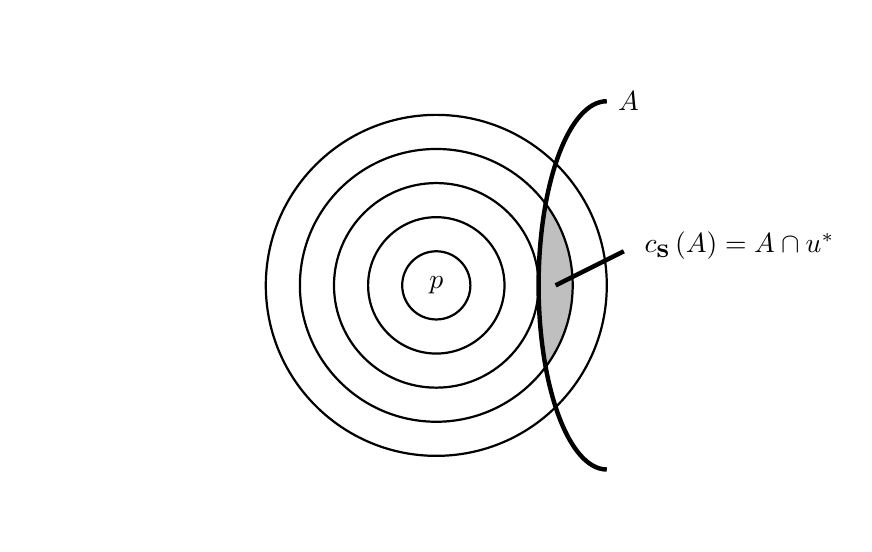
\begin{tikzpicture} [scale=\textwidth/14cm]

\definecolor{lightgray}{gray}{0.75};

% these coordinates guarantee the graph's total size
\node at (-6,3.5) [draw=none,fill=none, above right] { };
\node at (3.5,-3.5) [draw=none,fill=none, above right] { };

\begin{scope}
\clip (0,0) circle (2.0);
\fill[lightgray] (2.5,2.7) arc (90:270:1 and 2.7);
\end{scope}

%spheres
\begin{scope} [thick]
%inner sphere
\draw (0,0) circle (0.5)
  node {$p$};
%2nd sphere
\draw (0,0) circle (1.0);
%3rd sphere
\draw (0,0) circle (1.5);
%4th sphere
\draw (0,0) circle (2.0);
%5th sphere
\draw (0,0) circle (2.5);
\end{scope}

%new information
\begin{scope} [ultra thick]
\draw (2.5,2.7) node [right] {$\llbracket A\rrbracket$} arc (90:180:1 and 2.7) node [above=0.5cm,right=1.2cm,fill=white] {$c_{\textbf{s}}\left(A\right)=\llbracket A\rrbracket\cap u^*$} arc (180:270:1 and 2.7);

%line leading to caption
\draw (1.75,0) -- (2.75,0.5);
\end{scope}

\end{tikzpicture}
\caption{The possible worlds ``closest'' to the center $p$}\label{huber:fig1}
\end{figure}
% Here is where the onion ends

If we have a belief set $\cal B\subseteq L$ we can use a system of spheres $\textbf{s}$ in $w_{\cal L}$ that is centered on $\llbracket\begin{cal}B\end{cal}\rrbracket\subseteq w_{\cal L}$ to define a revision operator $*$ restricted to $\cal B$ as follows. For every sentence $A$ from $\cal L$:
$$\begin{cal}B\end{cal}*A=T\left(c_{\textbf{s}}\left(A\right)\right).$$
The idea is that what the ideal doxastic agent ends up believing after revising $*$ her old belief set $\cal B$ with the new information $A$ is (a set of sentences expressing) the proposition $c_{\textbf{s}}\left(A\right)$ that contains the possible worlds in $\llbracket A\rrbracket$ that are closest when the proposition expressed by her old belief set, $\llbracket\cal B\rrbracket$, is the center. Expansion is the special case where the proposition expressed by the new information properly overlaps with the proposition expressed by the old belief set, $\llbracket A\rrbracket\cap\llbracket\cal B\rrbracket\neq\emptyset$. In this special case the ideal doxastic agent does not have to leave the old center $\llbracket\cal B\rrbracket$ of her doxastic state; it suffices if she narrows it down to the possible worlds also contained in $\llbracket A\rrbracket$. However, in the general case of revision this intersection may be empty. In this general case the ideal doxastic agent may have to leave the innermost sphere $\llbracket\cal B\rrbracket$ and move to the smallest sphere $u^*$ that properly overlaps with $\llbracket A\rrbracket$ and adopt their intersection, $u^*\cap\llbracket A\rrbracket$, as the new center of her doxastic state.

As before we can picture the system of spheres centered on $\llbracket\cal B\rrbracket$ as an ``onion'' around $\llbracket\cal B\rrbracket$. The grey area $\llbracket\begin{cal}B\end{cal}*A\rrbracket=\llbracket T\left(c_{\textbf{s}}\left(A\right)\right)\rrbracket=u^*\cap\llbracket A\rrbracket$ is the logically strongest proposition the ideal doxastic agent believes after revising her old belief set $\cal B$ by the new information $A$; it is the new center of her doxastic state (\autoref{huber:fig2}).

% HERE IS WHERE THE ONION BEGINS
\begin{figure}[ht]
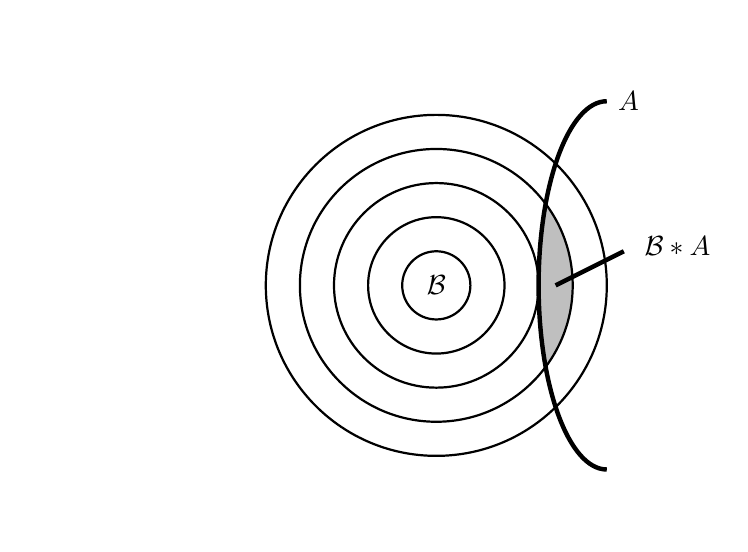
\begin{tikzpicture} [scale=\textwidth/14cm]

\definecolor{lightgray}{gray}{0.75};

% these coordinates guarantee the graph's total size
\node at (-6,3.5) [draw=none,fill=none, above right] { };
\node at (3.5,-3.5) [draw=none,fill=none, above right] { };

\begin{scope}
\clip (0,0) circle (2.0);
\fill[lightgray] (2.5,2.7) arc (90:270:1 and 2.7);
\end{scope}

%spheres
\begin{scope} [thick]
%inner sphere
\draw (0,0) circle (0.5)
  node {$\llbracket\begin{cal}B\end{cal}\rrbracket$};
%2nd sphere
\draw (0,0) circle (1.0);
%3rd sphere
\draw (0,0) circle (1.5);
%4th sphere
\draw (0,0) circle (2.0);
%5th sphere
\draw (0,0) circle (2.5);
\end{scope}

%new information
\begin{scope} [ultra thick]
\draw (2.5,2.7) node [right] {$\llbracket A\rrbracket$} arc (90:180:1 and 2.7) node [above=0.5cm,right=1.2cm,fill=white] {$\llbracket\begin{cal}B\end{cal}*A\rrbracket$} arc (180:270:1 and 2.7);

%line leading to caption
\draw (1.75,0) -- (2.75,0.5);
\end{scope}

\end{tikzpicture}
\caption{The strongest proposition believed after revising $\mathcal{B}$ by $A$}\label{huber:fig2}
\end{figure}
% Here is where the onion ends

\citet{g88} proves the following theorem which states that an ideal doxastic agent can be represented as revising her beliefs by relying on a system of spheres satisfying $\textbf{s}1$\,--\,$\textbf{s}4$ if, and only if, she can be represented as revising her beliefs by employing a revision function satisfying postulates $*1$\,--\,$*8$.

\begin{theorem}\label{th2}
Let $\cal L$ be a formal language, and let $w_{\cal L}$ be a set of possible worlds relative to which the sentences from $\cal L$ are interpreted and relative to which $\cal L$ is sufficiently rich. For each set of sentences $\cal B\subseteq L$ and each system of spheres $\textbf{s}$ in $w_{\cal L}$ that is centered on $\llbracket\cal B\rrbracket$ and satisfies $\textbf{s}1$\,--\,$\textbf{s}4$ there is a revision operator $*$ from $\left\{\cal B\right\}\times\cal L$ into $\powerset\!\left(\cal L\right)$ satisfying $*1$\,--\,$*8$ restricted to $\cal B$ such that for all $A\in\cal L$:
$$\begin{cal}B\end{cal}*A=T\left(c_{\textbf{s}}\left(A\right)\right).$$
For each revision operator $*$ from $\powerset\!\left(\cal L\right)\times\cal L$ into $\powerset\!\left(\cal L\right)$ satisfying $*1$\,--\,$*8$ and each set of sentences $\cal B\subseteq L$ there is a system of spheres $\textbf{s}$ in $w_{\cal L}$ that is centered on $\llbracket\cal B\rrbracket$ and satisfies $\textbf{s}1$\,--\,$\textbf{s}4$ such that for all $A\in\cal L$:
$$\begin{cal}B\end{cal}*A=T\left(c_{\textbf{s}}\left(A\right)\right).$$
\end{theorem}
The two representations of belief revision in terms of systems of spheres and in terms of belief revision functions are thus equivalent. Combined with \autoref{th1} this implies that the representation of belief revision in terms of systems of spheres and in terms of entrenchment orderings are also equivalent.%The conjunction of all the agent's beliefs is the most entrenched sentence that is not tautological. It expresses the proposition $\llbracket\cal B\rrbracket$ that is the center of her system of spheres.
%\pagebreak

As an aside let me note that \citepos{g88} notion of a system of spheres is more general than \citepos{l73} notion in the following respect. \citet{g88} allows $\textbf{s}$ to be centered on arbitrary propositions $p\subseteq w_{\cal L}$, whereas \citet[14f]{l73} requires the center $p$ to contain the actual world, and nothing but the actual world. These last two requirements are known as the principles of weak centering and of strong centering, respectively (see Briggs, \citethisvolume{thisvolume:briggs}). In another respect \citepos{g88} notion is less general than \citepos{l73}. This is so, because requirement $\textbf{s}4$ makes a doxastic version of the limit assumption, which \citet[19f]{l73} famously rejects and which \citet{h79} shows to be equivalent to the condition that the set of counterfactual consequences $\{C\in\begin{cal}L\end{cal}:A\boxright C\}$ of any consistent sentence $A$ be consistent. Ranking theory also makes a doxastic version of the limit assumption.

In the AGM theory of belief revision the ideal agent's old doxastic state is represented by her belief set $\cal B$ together with her entrenchment ordering $\preceq$ for $\cal B$. The latter ordering guides the revision process in that it specifies which elements of the old belief set are given up, and which are kept, when new information $D$ is received. The result of revising the old belief set by the new information $D$ is a new belief set $\begin{cal}B\end{cal}*D$. Sophia's old belief set $\cal B$ includes the beliefs that it will rain on Tuesday, that it will be sunny on Wednesday, and that weather forecasts are always right. Suppose her belief $A$ that it will be sunny on Wednesday is less entrenched than her belief $B$ that it will rain on Tuesday, which in turn is less entrenched than her belief $C$ that weather forecasts are always right, %$\alpha\wedge\neg\alpha\prec
$A\prec B\prec C$.

On Monday Sophia comes to believe that the weather forecast for Tuesday and Wednesday predicts rain, $D$. Consequently she has to give up her belief $A$ that it will be sunny on Wednesday or her belief $C$ that weather forecasts are always right. The reason is that it follows from $D$ that at least one of those two beliefs is false, i.e. $\left\{D\right\}\vdash\neg A\vee\neg C$. This implies that $A\wedge C\preceq\neg D$.
Since $A$ is less entrenched than $C$, i.e. $A\prec C$, $A$ has to go. Furthermore, since $\left\{C,D\right\}\not\vdash\neg B$ Sophia need not give up her belief $B$ that it will rain on Tuesday if she holds onto her belief $C$ that weather forecasts are always right, and adds the belief $D$ that the weather forecast for Tuesday and Wednesday predicts rain. In addition let us assume that $\neg D\prec B$ so that Sophia's entrenchment ordering looks as follows: where $X\sim Y$ is short for $X\preceq Y$ and $Y\preceq X$,
$$\bot\sim\neg A\prec A\sim A\wedge C\preceq\neg D\prec B\prec C\prec A\vee\neg A.$$
Thus Sophia's new belief set is
$$\begin{cal}B\end{cal}*D=Cn\left(\left\{X:\neg D\prec X\right\}\cup\left\{D\right\}\right)=Cn\left(\left\{B,C,D,\neg A\right\}\right).$$

To Sophia's surprise it is sunny on Tuesday after all. Therefore Sophia wants to revise her newly acquired belief set $\begin{cal}B\end{cal}*D$ a second time by $\neg B$ to correct her belief $B$ that it will rain on Tuesday. In addition, Sophia has to give up her belief $D$ that the weather forecast for Tuesday and Wednesday predicts rain (this might be because she has misheard the weather forecast) or her belief $C$ that weather forecasts are always right (this might be because she has been too gullible). The reason is that it follows from $\neg B$ that at least one of those two beliefs is false, i.e. $\left\{\neg B\right\}\vdash\neg D\vee\neg C$. Unfortunately AGM belief revision theory is of no help here. While Sophia could use her entrenchment ordering to revise her old belief set $\cal B$ to a new belief set $\begin{cal}B\end{cal}*D$, the entrenchment ordering itself has not been revised. Sophia's new doxastic state is silent as to whether $D$ is now more entrenched than $C$ (this might be because she was too gullible) or $C$ is now more entrenched than $D$ (this might be because she misheard the weather forecast) or $C$ is now as entrenched as $D$ (this might be because she was too gullible and misheard the weather forecast). However, the latter is exactly the kind of information that Sophia needs in order to revise her beliefs a second time.


\section{Iterated Belief Revision}

More generally, the problem is that Sophia's doxastic state is represented as a belief set plus an entrenchment ordering before the revision process, but as a belief set without an entrenchment ordering after the revision process. To handle \emph{iterated} belief revisions the ideal agent's doxastic state has to be represented in the same way before and after the revision process. \citet[37]{gr95} call this the ``principle of categorical matching.''

\citet{n94}, \citet{b96}, \citet{dp97}, \citet{s98}, \citet{f00}, \citet{r03}, \citet{r06}, and others do exactly this (see also Caie, \citethisvolume{thisvolume:caie}, Section 2.4). They augment the AGM postulates by additional postulates specifying how the ideal doxastic agent should revise her entrenchment ordering in addition to her belief set when she receives new information. On their accounts the ideal agent's doxastic state is represented as a belief set plus an entrenchment ordering both before and after the revision process, and both of these two elements are revised when new information is received.

Let us have a closer look at the proposal by \citet{dp97} (Caie, \citethisvolume{thisvolume:caie}, Section 2.4 also discusses \citealt{b96}'s proposal). In addition to postulates $*1$\,--\,$*8$ they propose four more postulates for iterated belief revision. The first of these, $*9$, says that revising an old belief set by new information (say, a conjunction) should result in the same new belief set as first revising the old belief set by a logical consequence of the new information (say, one of the two conjuncts) and then revising the resulting belief set by the new information in its entirety. That is, revision by a more specific piece of information such as that Sophia had red wine should override all changes that result from first revising the old belief set by a less specific piece of information such as that Sophia had wine.

The second of these new postulates, $*10$, says that revising an old belief set consecutively by two pieces of information that are logically inconsistent should result in the same new belief set as revising the old belief set by the second piece of information alone. That is, revision by the second piece of information---say, that Sophia had red wine---should override all changes that result from first revising the old belief by the first piece of information that is logically incompatible with the second piece of information---say, that Sophia had no wine.

Next suppose the ideal doxastic agent holds a belief after revising her old belief set by a piece of information. This may, but need not be a new belief, i.e. a belief not held previously. The third new postulate, $*11$, says that the ideal doxastic agent should also hold this belief if she first revises her old belief set by this very belief and then revises the resulting belief set by said piece of information.

Finally, suppose there is a sentence that is logically compatible with the result of revising the ideal doxastic agent's old belief set by a piece of information. The fourth new postulate, $*12$, says that this sentence should also be logically compatible with what the ideal doxastic agent ends up believing if she first revises her old belief set by this very sentence and then revises the resulting belief set by said piece of information.

More precisely, \citet{dp97} require the following of all sets of sentences $\cal B\subseteq L$ and all sentences $A$ and $B$ from $\cal L$:
\begin{enumerate}
\item[$*$9.] If $\left\{A\right\}\vdash B$, then $\left(\begin{cal}B\end{cal}*B\right)*A=\begin{cal}B\end{cal}*A$.
\item[$*$10.] If $\left\{A\right\}\vdash\neg B$, then $\left(\begin{cal}B\end{cal}*B\right)*A=\begin{cal}B\end{cal}*A$.
\item[$*$11.] If $B\in\begin{cal}B\end{cal}*A$, then $B\in\left(\begin{cal}B\end{cal}*B\right)*A$.
\item[$*$12.] If $\neg B\not\in\begin{cal}B\end{cal}*A$, then $\neg B\not\in\left(\begin{cal}B\end{cal}*B\right)*A$.
\end{enumerate}
In order to represent these four new postulates more perspicuously it will be helpful to consider the following reformulation of a system of spheres $\textbf{s}$ in $w_{\cal L}$ centered on some proposition $p$.

Let $p\subseteq w_{\cal L}$ be a proposition and let $\leq$ be a binary relation on $w_{\cal L}$. The relation $\leq$ is an \emph{implausibility ordering} on $w_{\cal L}$ with center $p$ just in case the following holds for all possible worlds $\omega$, $\omega'$, and $\omega''$ from $w_{\cal L}$ and all propositions $q\subseteq w_{\cal L}$:
\begin{enumerate}
\item[$\leq$1.] $\omega\leq\omega'$ or $\omega'\leq\omega$.\hfill $\leq$ is connected
\item[$\leq$2.] If $\omega\leq\omega'$ and $\omega'\leq\omega''$, then $\omega\leq\omega''$.\hfill $\leq$ is transitive
\item[$\leq$3.] $\omega\in p$ if, and only if, for all $\omega^*\in w_{\cal L}:\omega\leq\omega^*$.
\item[$\leq$4.] If $q\neq\emptyset$, then $\left\{\omega\in q:\omega\leq\omega^*\mbox{ for all }\omega^*\in q\right\}\neq\emptyset$.
\end{enumerate}
As suggested by its name, an implausibility ordering on $w_{\cal L}$ with center $p$ orders the possible worlds from $w_{\cal L}$ according to their implausibility. Among other things, it is required that any two possible worlds can be compared with respect to their implausibility: either the first possible world is at least implausible as the second possible world, or the second possible world is at least as implausible as the first possible world, or both. It is also required that the ordering is transitive: if one possible world is at least as implausible as a second possible world, and the second possible world is at least as implausible as a third possible world, then the first possible world is at least as implausible as the third possible world.

Furthermore it is required that the possible worlds in the center are no more implausible than all possible worlds. That is, the center is the proposition that contains all and only the least implausible possible worlds. Finally it is required that each proposition that contains a possible world also contains a possible world that is no more implausible than all possible worlds in this proposition. The latter feature allows us to identify the implausibility of a non-empty or logically consistent proposition with the implausibility of the least implausible possible world(s) comprised by this proposition.

A system of spheres centered on $p$ can be understood as an implausibility ordering with the center $p$ containing the least implausible possible worlds. In terms of such an implausibility ordering the problem with the original AGM approach is the following. Before the revision process the ideal agent's doxastic state is represented as a belief set $\cal B$ plus an implausibility ordering $\leq_{\cal B}$ with center $\llbracket\cal B\rrbracket$. After revision by the new information $A$ the ideal agent's doxastic state is represented as a belief set $\begin{cal}B\end{cal}*A$, but without a corresponding implausibility ordering $\leq_{\begin{cal}B\end{cal}*A}$. \citepos{gr95} principal of categorical matching urges us to represent the ideal agent's doxastic state as a belief set plus an implausibility ordering both before and after the revision process. In these terms \citepos{dp97} postulates $*9$\,--\,$*12$ become the following simple requirements.

First, the implausibility ordering among the possible worlds within the proposition expressed by the new information should be the same before and after a revision by the new information. Second, the implausibility ordering among the possible worlds outside of the proposition expressed by the new information should also be the same before and after a revision by the new information. Third, if a possible world within the proposition expressed by the new information is less implausible than a possible world outside of this proposition before revision by the new information, then this should remain so after a revision by the new information. Fourth, if a possible world within the proposition expressed by the new information is at least as implausible as a possible world outside of this proposition before revision by the new information, then this should also remain so after a revision by the new information. That is, where $\omega<\omega'$ holds for arbitrary possible worlds $\omega$ and $\omega'$ from $w_{\cal L}$ if, and only if, $\omega\leq\omega'$ and $\omega'\not\leq\omega$, the following is required of all possible worlds $\omega$ and $\omega'$ from $w_{\cal L}$ and all sentences $A$ from $\cal L$:
\begin{enumerate}
\item[$\leq$5.] If $\omega,\omega'\in\llbracket A\rrbracket$, then: $\omega\leq_{\cal B}\omega'$ just in case $\omega\leq_{\begin{cal}B\end{cal}*A}\omega'$.
\item[$\leq$6.] If $\omega,\omega'\not\in\llbracket A\rrbracket$, then: $\omega\leq_{\cal B}\omega'$ just in case $\omega\leq_{\begin{cal}B\end{cal}*A}\omega'$.
\item[$\leq$7.] If $\omega\in\llbracket A\rrbracket$ and $\omega'\not\in\llbracket A\rrbracket$ and if $\omega<_{\cal B}\omega'$, then $\omega<_{\begin{cal}B\end{cal}*A}\omega'$.
\item[$\leq$8.] If $\omega\in\llbracket A\rrbracket$ and $\omega'\not\in\llbracket A\rrbracket$ and $\omega\leq_{\cal B}\omega'$, then $\omega\leq_{\begin{cal}B\end{cal}*A}\omega'$.
\end{enumerate}
Before we turn to a representation theorem for iterated belief revision let us consider a third representation theorem for belief revision. \autoref{th1} and \autoref{th2} tell us that the representation of belief revision in terms of entrenchment orderings, in terms of belief revision functions, and in terms of systems of spheres are all equivalent. According to the following theorem due to \citet{g88} this equivalence extends to the representation of belief revision in terms of implausibility orderings.
\begin{theorem}\label{th3}
Let $\cal L$ be a formal language, and let $w_{\cal L}$ be a set of possible worlds relative to which the sentences from $\cal L$ are interpreted and relative to which $\cal L$ is sufficiently rich. For each set of sentences $\cal B\subseteq L$ and each implausibility ordering $\leq$ on $w_{\cal L}$ with center $\llbracket\cal B\rrbracket$ that satisfies $\leq\!\!1$\,--\,$\leq\!\!4$ there is a revision operator $*$ from $\left\{\cal B\right\}\times\cal L$ into $\powerset\!\left(\cal L\right)$ satisfying $*1$\,--\,$*8$ restricted to $\cal B$ such that for all $A\in\cal L$:
$$\begin{cal}B\end{cal}*A=T\left(\left\{\omega\in\llbracket A\rrbracket:\omega\leq\omega^*\mbox{ for all }\omega^*\in\llbracket A\rrbracket\right\}\right).$$
For each revision operator $*$ from $\powerset\!\left(\cal L\right)\times\cal L$ into $\powerset\!\left(\cal L\right)$ that satisfies $*1$\,--\,$*8$ and each set of sentences $\cal B\subseteq L$ there is an implausibility ordering $\leq$ on $w_{\cal L}$ with center $\llbracket\cal B\rrbracket$ satisfying $\leq\!\!1$\,--\,$\leq\!\!4$ such that for all $A\in\cal L$:
$$\begin{cal}B\end{cal}*A=T\left(\left\{\omega\in\llbracket A\rrbracket:\omega\leq\omega^*\mbox{ for all }\omega^*\in\llbracket A\rrbracket\right\}\right).$$
\end{theorem}
The complicated looking proposition $\left\{\omega\in\llbracket A\rrbracket:\omega\leq\omega^*\mbox{ for all }\omega^*\in\llbracket A\rrbracket\right\}$ is simply the set of the least implausible possible worlds in which the new information $A$ is true. This means that the belief set $\begin{cal}B\end{cal}*A$ that results from revising $*$ the ideal doxastic agent's old belief set $\cal B$ by new information $A$ expresses the proposition that is comprised by the least implausible $A$-worlds.

Against this background we can now state the following representation theorem for iterated belief revision due to \citet{dp97}. According to it the representation of iterated belief revision in terms of belief revision functions \`{a} la postulates $*9$\,--\,$*12$ is equivalent to the simple representation of iterated belief revision in terms of implausibility orderings \`{a} la $\leq\!\!5$\,--\,$\leq\!\!8$.
\begin{theorem}\label{th4}
Let $\cal L$ and $w_{\cal L}$ be as in \autoref{th3}. Suppose $*$ is a revision operator from $\powerset\!\left(\cal L\right)\times\cal L$ into $\powerset\!\left(\cal L\right)$ that satisfies $*1$\,--\,$*8$. According to \autoref{th3}, there exists a family of implausibility orderings $\left(\leq_{\cal B}\right)_{\cal B\subseteq L}$ on $w_{\cal L}$ such that for each set of sentences $\cal B\subseteq L$: $\leq_{\cal B}$ satisfies $\leq\!\!1$\,--\,$\leq\!\!4$ and is such that, for all sentences $A\in\cal L$, $\begin{cal}B\end{cal}*A=T\left(\left\{\omega\in\llbracket A\rrbracket:\omega\leq_{\cal B}\omega^*\mbox{ for all }\omega^*\in\llbracket A\rrbracket\right\}\right)$. For this $*$ and any one of these families $\left(\leq_{\cal B}\right)_{\cal B\subseteq L}$: $*$ satisfies $*9$\,--\,$*12$ if, and only if, for every set of sentences $\cal B\subseteq L$, $\leq_{\cal B}$ satisfies $\leq\!\!5$\,--\,$\leq\!\!8$.
%Suppose $*$ is a function from $\powerset\left(\cal L\right)\times\cal L$ into $\powerset\left(\cal L\right)$ satisfying $*1$-$*8$. Suppose further $\leq_{\cal B}$ is the corresponding implausibility ordering on $w_{\cal L}$ with center $\llbracket\cal B\rrbracket$ satisfying $\leq1$-$\leq4$ and, for all $A\in\cal L$, $\begin{cal}B\end{cal}*A=T\left(\left\{\omega\in\llbracket A\rrbracket:\omega\leq\omega^*\mbox{ for all }\omega^*\in\llbracket A\rrbracket\right\}\right)$. Then: $*$ satisfies $*9$-$*12$ if, and only if, $\leq_{\cal B}$ satisfies $\leq 5$-$\leq 8$.
\end{theorem}
The approaches to iterated belief revision mentioned above all have in common that the ideal agent's doxastic state is represented as a belief set plus an entrenchment ordering/system of spheres/implausibility ordering both before and after the revision process. Furthermore these approaches have in common that the new information is represented as a single sentence (or a single proposition). The latter is also true for the approach by \citet{jt07} discussed below, but not for what \citet{r09} calls ``two-dimensional'' belief revision operators (see also \citealt{c97,fr04,r07}).

In one-dimensional belief revision, as we may call it, the new information comes as a ``naked'' \citep{r07} sentence or proposition. It is the job of the various belief revision methods, as opposed to the new information itself, to say exactly where in the new entrenchment ordering/system of spheres/implausibility ordering the new sentence or proposition should be placed. These belief revision methods include lexicographic revision \citep{n94}, natural revision \citep{b96}, irrevocable revision \citep{s98, f00}, irrefutable revision \citep{r06}, and still others. In two-dimensional belief revision it is the new information itself that carries at least part of this information. Here the new information does not say \emph{that} the input sentence $A$ is \emph{true} (so should be accepted according to the Success postulate). Instead it specifies, at least to some extent, \emph{how firmly} $A$ is \emph{accepted} or \emph{believed} by specifying that, in the new entrenchment ordering $\preceq^*$, $A$ is at least as entrenched as some ``reference sentence'' $B$. Thus the new information is now of the form: $A\preceq^* B$. (For the purposes of this entry we may ignore ``non-prioritized'' belief revision, where the new information need not be accepted. See \citealp{hfcf01}.)

Let us return to our example. On Monday Sophia comes to believe that the weather forecast for Tuesday and Wednesday predicts rain, $D$. In one-dimensional belief revision she picks one of the iterated belief revision methods mentioned above. Then she revises her old belief set $\cal B$ and entrenchment ordering $\preceq_{\cal B}$ to obtain a new belief set $\begin{cal}B\end{cal}*D$ and a new entrenchment ordering $\preceq_{\begin{cal}B\end{cal}*D}$. Different methods return different outputs, but on all of them Sophia ends up believing that it will rain on Tuesday, $B$. On Tuesday Sophia sees that it is sunny and so receives the new information that it does not rain after all, $\neg B$. In one-dimensional belief revision Sophia proceeds as before.

In two-dimensional belief revision Sophia does not receive the qualitative information $\neg B$ about Tuesday's weather. Instead she receives the comparative information $C\preceq^*\neg B$ about her new doxastic state. This piece of new information says that, in her new entrenchment ordering $\preceq^*$, the claim that it does not rain on Tuesday is at least as entrenched as the claim that weather forecasts are always right, indicating that she trusts her sight at least as much as the weatherperson (we could take a reference sentence other than $C$).

Now, there still are several belief revision methods to choose from (see \citealt{r09}). Among others, this reflects the fact that Sophia can respect the constraint $C\preceq^*\neg B$ by lowering the doxastic status of $C$, or by raising the doxastic status of $\neg B$. However, the new information now is more specific and leaves less room to be filled by the revision method. It is then only a small, but crucial step to equip Sophia with the quantitative, numerical information that $\neg B$ is entrenched to a specific degree. In this case the new information completely determines exactly where $\neg B$ is located in the new entrenchment ordering on its own, without the help of the revision method. The latter merely has to incorporate this new information into Sophia's old doxastic state in a consistent way. Ranking theory does exactly this.

%\textcolor{orange}{She revises her old belief set $\cal B$ by the new information $\gamma\preceq \delta$ to obtain the new belief set $\cal B*_{\gamma}\delta$ as well as a new entrenchment ordering $\preceq_{\gamma\preceq\delta}$. Since the entrenchment ordering has been updated as well she can use it to determine that $\gamma$ is more entrenched than $\delta$, and thus she can revise $\cal B*_{\gamma}\delta$ by $\neg\beta\preceq\neg\beta$.}

Before presenting ranking theory let us return to the qualitative approaches to iterated belief revision. Postulates $*1$\,--\,$*12$ are still compatible with many conflicting belief revision methods. \citet{jt07} attempt to remedy this situation by additionally requiring the ideal doxastic agent to consider the new information $B$ to be \emph{independent} of a sentence $A$ after revision by $B$ if she considered $B$ to be independent of $A$ before revision by $B$. In other words, revision should preserve independencies. While the idea behind \citet{jt07}'s proposal seems to be correct, their actual requirement turns out to be too strong. The reason is that their notion of dependence is too strong in the sense that too many sentences are rendered independent of other sentences.

According to \citet{jt07} a believed sentence $A$ is independent of another sentence $B$ if the believed sentence $A$ is still believed after revision by the negation of the other sentence, $\neg B$. However, I can receive new information $\neg B$---say, that the captain of my favorite soccer team will not be fit for the match---whose negation $\neg\neg B$ is positively relevant to, and so \emph{not} independent of, a belief of mine $A$---say, that my favorite soccer team will win the match---without making me give up this belief of mine altogether. More generally, the ways two sentences can depend on each other are many and varied, and the qualitative and comparative notions of AGM belief revision theory and its refinements seem to be too coarse-grained to capture these dependencies. \citet{hs08} argue axiomatically, and we will see in the next section, that, in order to adequately represent all dependencies, and to handle iterated belief revisions, one has to go all the way from qualitative belief sets and comparative entrenchment orderings/systems of spheres/implausibility orderings to quantitative, numerical ranking functions.

%\footnote{\textcolor{red}{Space does not permit a thorough discussion of iterated belief revision, which has been the topic of recent research. The interested reader is referred to, among others, Bonanno (2012), Hansson (2012), Ramachandran \& Nayak \& Orgun (2012), Rott (2011), Weydert (2012), and, especially, the survey in \citet{r09}.}}


\section{Ranking Theory}

Ranking functions are introduced by \citet{s88,s90} to represent qualitative conditional belief. A comprehensive overview can be found in \citet{s12}. The theory is quantitative or numerical in the sense that ranking functions assign numbers, so-called \emph{ranks}, to sentences or propositions. These numbers are needed for the definition of conditional ranking functions which represent conditional beliefs. As we will see, once conditional ranking functions are defined we can interpret everything in purely qualitative, albeit conditional terms. The numbers assigned by conditional ranking functions are called \emph{conditional ranks}. They are defined as differences of non-conditional ranks.%Since conditional ranks are defined as differences of non-conditional ranks, this may explain why ranks are measured on an interval scale \citep{klst71}.

Instead of taking the objects of belief to be sentences of a formal language it is both more general and more convenient to take them to be propositions of some field or algebra over a set of possible worlds $W$. Here is the relevant definition. A set of subsets of $W$, $\begin{cal}A\end{cal}\subseteq\powerset\!\left(W\right)$, is an \emph{algebra over $W$} if, and only if,
\begin{enumerate}
\item[(i)] the empty or contradictory set $\emptyset$ is a proposition in $\cal A$,
\item[(ii)] if $A$ is a proposition in $\cal A$, then the complement or negation of $A$, $W\setminus A=\overline{A}$, is also a proposition in $\cal A$, and
\item[(iii)] if both $A$ and $B$ are propositions in $\cal A$, then the union or disjunction of $A$ and $B$, $A\cup B$, is also a proposition in $\cal A$.
\end{enumerate}
%We say that a
An algebra $\cal A$ over $W$ is a \emph{$\sigma$-algebra} if, and only if, the following holds for every countable set $\begin{cal}B\end{cal}\subseteq\powerset\!\left(W\right)$: if all the members or elements of $\begin{cal}B\end{cal}$ are propositions in $\cal A$, i.e. if $\cal B\subseteq A$, then the union or disjunction of the elements of $\cal B$, $\bigcup\cal B$, is also a proposition in $\cal A$. Finally, %we say that
an algebra $\cal A$ over $W$ is \emph{complete} if, and only if, the following holds for every (countable or uncountable) set $\begin{cal}B\end{cal}\subseteq\powerset\!\left(W\right)$: if all the members or elements of $\begin{cal}B\end{cal}$ are propositions in $\cal A$, i.e. if $\cal B\subseteq A$, then the union or disjunction of the elements of $\cal B$, $\bigcup\cal B$, is also a proposition in $\cal A$. The power-set of a set of possible worlds $W$, $\powerset\!\left(W\right)$, is a complete algebra over $W$.
%If we have a formal language $\cal L$ and $w_{\cal L}$ is the set of all models or truth-value assignments of $\cal L$, then $\begin{cal}A\end{cal}=\left\{\llbracket A\rrbracket\subseteq w_{\cal L}:A\in\cal L\right\}$ is an algebra of propositions over $w_{\cal L}$. $\sigma\left(\cal A\right)$ is the $\sigma$- algebra generated by $\cal A$ ($\sigma\left(\cal A\right)$ is the intersection of all $\sigma$- algebras containing $\cal A$ as a subset). $\gamma\left(\cal A\right)$ is the complete algebra generated by $\cal A$ ($\gamma\left(\cal A\right)$ is the intersection of all complete algebras containing $\cal A$ as a subset). So for every formal language of sentences there is an algebra of propositions over the set of models of the formal language. Since the converse is not true, the semantic framework of propositions is more general than the syntactic framework of sentences (for more on the relation between ranking functions on formal languages and ranking functions on algebras of propositions see Huber 2006).
%As will become clear, it is also more convenient. Consider a set of possible worlds $W$ and an algebra of propositions $\cal A$ over $W$.

A function $\varrho:\begin{cal}A\end{cal}\rightarrow\mathbb{N}\cup\left\{\infty\right\}$ from an algebra of propositions $\cal A$ over a non-empty set of possible worlds $W$ into the set of natural numbers $\mathbb{N}$ extended by infinity $\infty$, $\mathbb{N}\cup\left\{\infty\right\}$, is a \emph{%finitely / countably / completely minimitive
ranking function} on $\cal A$ just in case for %all finite / countable / arbitrary sets of propositions $\begin{cal}B\end{cal}\subseteq\begin{cal}A\end{cal}$
all propositions $A$ and $B$ from $\cal A$:
\begin{eqnarray}
\varrho\left(W\right)&=&0,\label{rank1}\\
\varrho\left(\emptyset\right)&=&\infty,\label{rank2}\\
\varrho\left(A\cup B\right)&=&\min\left\{\varrho\left(A\right),\varrho\left(B\right)\right\}.\label{rank3}
\end{eqnarray}
As in probability theory, if $\cal A$ is a $\sigma$-algebra, axiom (\ref{rank3}) can be strengthened to countable unions. The resulting ranking function is called ``countably minimitive.'' In contrast to probability theory, if $\cal A$ is a complete algebra, axiom (\ref{rank3}) can even be strengthened to arbitrary unions. The resulting ranking function is called ``completely minimitive.''

For a non-empty or consistent proposition $A\neq\emptyset$ from $\cal A$ the conditional ranking function $\varrho\left(\cdot\mid A\right):\begin{cal}A\end{cal}\setminus\left\{\emptyset\right\}\rightarrow\mathbb{N}\cup\left\{\infty\right\}$ based on the (non-conditional) ranking function $\varrho\left(\cdot\right):\begin{cal}A\end{cal}\rightarrow\mathbb{N}\cup\left\{\infty\right\}$ is defined as
\[\varrho\left(\cdot\mid A\right)=\left\{\begin{array}{l}\varrho\left(\cdot\cap A\right)-\varrho\left(A\right),\quad\mbox{if}\quad\varrho\left(A\right)<\infty,\\
\infty\mbox{ or }0,\hfill\mbox{if}\quad\varrho\left(A\right)=\infty.\end{array}\right.\]
For the case where $\varrho\left(A\right)=\infty$ \citet[63]{gj96} suggest $\infty$ as the value for $\varrho\left(B\mid A\right)$ for all propositions $B$ from $\cal A$. For this case \citet[464]{h06} suggests $0$ as the value for $\varrho\left(B\mid A\right)$ for all non-empty or consistent propositions $B$ from $\cal A$ and additionally stipulates $\varrho\left(\emptyset\mid A\right)=\infty$ to ensure that every conditional ranking function on $\cal A$ is a ranking function on $\cal A$. %Stipulating $\varrho\left(\emptyset\mid A\right)=\infty$ ensures that every conditional ranking function is a ranking function on $\cal A$.

A ranking function $\varrho$ is \emph{regular} if, and only if,
$$\varrho\left(A\right)<\varrho\left(\emptyset\right)=\infty,$$
for all non-empty or consistent propositions $A$ from $\cal A$. In contrast to probability theory it is always possible to define a regular ranking function, no matter how rich or fine-grained the underlying algebra of propositions (see \citealp{hun}).

Ranks are interpreted doxastically as grades of disbelief. A proposition $A$ is disbelieved just in case $A$ is assigned a positive rank, $\varrho\left(A\right)>0$. A proposition that is not disbelieved is assigned rank $0$, but this does not mean that it is believed. Instead, belief in a proposition is characterized as disbelief in its negation: a proposition $A$ is believed just in case the negation of $A$, $\overline{A}$, is disbelieved, $\varrho\left(\overline{A}\right)>0$. An agent suspends judgment with respect to a proposition (and its negation) if, and only if, both the proposition and its negation are assigned rank $0$.

A proposition $A$ is disbelieved conditional on a proposition $C$ just in case $A$ is assigned a positive rank conditional on $C$, $\varrho\left(A\mid C\right)>0$. A proposition $A$ is believed conditional on a proposition $C$ just in case the negation of $A$, $\overline{A}$, is disbelieved conditional on $C$, $\varrho\left(\overline{A}\mid C\right)>0$. It takes getting used to read positive numbers in this ``negative'' way, but mathematically this is the simplest way to axiomatize ranking functions.

Note that it follows from \citepos{h06} definition of a conditional ranking function that the ideal doxastic agent should not disbelieve a proposition $A$ conditional on itself, $\varrho\left(A\mid A\right)=0$, if, and only if, $A$ is non-empty or consistent.

In doxastic terms the first axiom says that the ideal doxastic agent should not disbelieve the tautological proposition $W$. The second axiom says that she should disbelieve the empty or contradictory proposition $\emptyset$ with maximal strength $\infty$. Given the definition of conditional ranks, the second axiom can also be read in purely qualitative, albeit conditional terms: in these terms it says that the ideal doxastic agent should disbelieve the empty or contradictory proposition conditional on any non-empty or consistent proposition. It follows that the ideal doxastic agent should believe the tautological proposition with maximal strength, or conditional on any non-empty or consistent proposition.

Part of what the third axiom says is that the ideal doxastic agent should %unconditionally
disbelieve a disjunction $A\cup B$ just in case she %unconditionally
disbelieves both its disjuncts $A$ and $B$. Given the definition of conditional ranks, the third axiom extends this requirement to conditional beliefs. As noted above, the ideal doxastic agent should not disbelieve a non-empty or consistent proposition conditional on itself. Given this consequence of the definition of a conditional ranking function, the third axiom says---in purely qualitative, albeit conditional terms---the following. For all non-empty or consistent propositions $C$, the ideal doxastic agent should disbelieve a disjunction $A\cup B$ conditional on $C$ just in case she disbelieves $A$ conditional on $C$ and she disbelieves $B$ conditional on $C$. Countably and completely minimitive ranking functions extend this ``conditional consistency'' requirement to countable and arbitrary unions, respectively. For any non-empty or consistent proposition $C$, the ideal doxastic agent should disbelieve $\bigcup\cal B$ conditional on $C$ just in case she disbelieves each disjunct $B$ from $\cal B$ conditional on $C$. We thus see that all that axioms (\ref{rank1})--(\ref{rank3}) of ranking theory ask of the ideal doxastic agent is that her beliefs be consistent, and that her conditional beliefs be conditionally consistent.

Ranks are numerical, but unlike probabilities, which are measured on an absolute scale, ranks do not utilize all the information carried by these numbers. Instead, ranks are at best measured on a ratio scale \citep{hs08}---at best, because even the choice of $0$ as threshold for disbelief is somewhat arbitrary, as \citet[9]{s15} notes (but see \citealp{r18}, for subtle differences for conditional belief). Some positive, but finite natural number would do just as well. This is perhaps most perspicuous by considering what \citet{s12} calls the \emph{two-sided} ranking function $\beta:\begin{cal}A\end{cal}\rightarrow\mathbb{Z}\cup\left\{\infty\right\}\cup\left\{-\infty\right\}$ whose range is the set of integers $\mathbb{Z}$ extended by plus infinity $\infty$ and minus infinity $-\infty$, $\mathbb{Z}\cup\left\{\infty\right\}\cup\left\{-\infty\right\}$. $\beta$ is defined in terms of $\varrho$ as follows: for all propositions $A$ in $\cal A$, $\beta\left(A\right)=\varrho\left(\overline{A}\right)-\varrho\left(A\right)$. Ranking functions and two-sided ranking functions are interdefinable. The latter are more difficult to axiomatize, but they may be more intuitive, because they characterize belief in positive terms as follows.

A proposition $A$ is believed if, and only if, its two-sided rank is positive, $\beta\left(A\right)>0$. A proposition $A$ is believed conditional on a proposition $C$ if, and only if, its two-sided conditional rank is positive, $\beta\left(A\mid C\right)>0$. Interestingly, any other finite threshold equally gives rise to a notion of belief (that is consistent and deductively closed as explained below): a proposition is believed if, and only if, its rank is greater than some finite, non-negative threshold $n$, $\beta\left(A\right)>n$. Hence ranking theory validates the Lockean thesis \citep{f09, h09a}. Furthermore, while it may appear unfair to reserve infinitely many numbers for belief and for disbelief, and only the number $0$ for suspension of judgment, we now see that this is not essential to the theory and can be fixed by adopting a threshold other than $0$ (there are still only finitely many levels for suspension of judgment, though).

Doxastically interpreted, axioms (\ref{rank1})--(\ref{rank3}) are synchronic norms for how an ideal doxastic agent should organize her beliefs and conditional beliefs at a given moment in time. These axioms are supplemented by diachronic norms for how she should update her beliefs and conditional beliefs over time if new information of various formats is received. The first update rule is defined for the case where the new information comes in the form a certainty. It mirrors the update rule of strict conditionalization from probability theory \citep{v00}.
\newtheorem{update}{Update Rule}
\begin{update}[Plain Conditionalization, \citealt{s88}]\label{rankrule1}
If $\varrho\left(\cdot\right):\begin{cal}A\end{cal}\rightarrow\mathbb{N}\cup\left\{\infty\right\}$ is the ideal doxastic agent's ranking function at time $t$, and between $t$ and the later time $t'$ her ranks for $E$ and $\overline{E}$ from $\begin{cal}A\end{cal}$ are directly affected and she becomes certain of $E$, but no logically stronger proposition (i.e. her rank for $E$ at $t$ is finite, and $E$ is the logically strongest proposition for whose negation $\overline{E}$ her rank at $t'$ is $\infty$), and her ranks are not directly affected in any other way such as forgetting etc., then her ranking function at $t'$ should be $\varrho_E\left(\cdot\right)=\varrho\left(\cdot\mid E\right)$.
\end{update}
Plain conditionalization asks the ideal doxastic agent to revise her beliefs and conditional beliefs by holding onto those conditional beliefs whose condition is the most specific, i.e. logically strongest, proposition she became certain of, subject to the constraint that the beliefs and conditional beliefs in the resulting new belief set are consistent and conditionally consistent, respectively. In slightly different terminology we can say that plain conditionalization has the ideal agent revise her doxastic state by holding onto those inferential beliefs whose premise is the logically strongest proposition she became certain of as a result of some experiential event that is not under her doxastic control.

The second update rule is defined for the case where the new information comes in the form of new ranks for the elements of a partition. It mirrors the update rule of Jeffrey conditionalization from probability theory \citep{j83}.
\begin{update}[Spohn Conditionalization, \citealt{s88}]\label{rankrule2}
If $\varrho\left(\cdot\right):\begin{cal}A\end{cal}\rightarrow\mathbb{N}\cup\left\{\infty\right\}$ is the ideal doxastic agent's ranking function at time $t$, and between $t$ and the later time $t'$ her ranks on the experiential partition $\left\{E_i\in\begin{cal}A\end{cal}:i\in I\right\}$ are directly affected and change \textbf{to} $n_i\in\mathbb{N}\cup\left\{\infty\right\}$ with $\min\left\{n_i:i\in I\right\}=0$, and $n_i=\infty$ if $\varrho\left(E_i\right)=\infty$, and her %finite
ranks are not directly affected on any finer partition or in any other way such as forgetting etc., then her ranking function at $t'$ should be $\varrho_{E_i\rightarrow n_i}\left(\cdot\right)$,
$$\varrho_{E_i\rightarrow n_i}\left(\cdot\right)=\min{_{i\in I}}\left\{\varrho\left(\cdot\mid E_i\right)+n_i\right\}.$$
\end{update}
Spohn conditionalization asks the ideal doxastic agent to revise her beliefs and conditional beliefs by holding onto those conditional beliefs whose conditions are the most specific propositions whose doxastic standing has changed as a result of some experiential event that is not under her doxastic control, subject to the constraint that the beliefs and conditional beliefs in the resulting new belief set are consistent and conditionally consistent, respectively. The restriction to hold fixed only those conditional beliefs whose conditions are the most specific propositions whose doxastic standing has been directly affected is important.

Suppose you hold the conditional beliefs that Sophia will have white wine tonight if there is wine left, and that she will have red wine tonight if there is red wine left, but no white wine---say, because you believe that Sophia prefers having white wine to having red wine to having no wine. Suppose further you subsequently come to believe, as a result of being told so by a source you deem reliable, that there is red wine left, but no white wine. Since your beliefs are deductively closed you also come to believe that there is wine left. In this case you should \emph{not} hold onto your conditional belief that Sophia will have white wine tonight if there is wine left. Instead, you should only hold onto your conditional belief that Sophia will have red wine tonight if there is red wine left, but no white wine. The same is true if you subsequently do not merely come to believe, but become certain in this way that there is red wine left, but no white wine. This is the reason for the restriction in plain conditionalization to hold fixed only those conditional beliefs whose condition is the logically strongest proposition the ideal doxastic agent becomes certain of. Furthermore, this illustrates that plain conditionalization is the special case of Spohn conditionalization where the experiential partition is $\left\{E,\overline{E}\right\}$ and where the new ranks are $0$ and $\infty$, respectively.

The third update rule is defined for the case where the new information reports the differences between the old and the new ranks for the elements of a partition. It mirrors the update rule of Field conditionalization from probability theory \citep{f78} and is developed further in \citet{b13} .
\begin{update}[Shenoy Conditionalization, \citealt{s91}]\label{rankrule3}
If $\varrho\left(\cdot\right):\begin{cal}A\end{cal}\rightarrow\mathbb{N}\cup\left\{\infty\right\}$ is the ideal doxastic agent's ranking function at time $t$, and between $t$ and the later time $t'$ her ranks on the experiential partition $\left\{E_i\in\begin{cal}A\end{cal}:i\in I\right\}$ are directly affected and change \textbf{by} $z_i\in\mathbb{N}$, where $\min\left\{z_i:i\in I\right\}=0$, and her %finite
ranks are not directly affected on any finer partition or in any other way such as forgetting etc., then her ranking function at $t'$ should be $\varrho_{E_i\uparrow z_i}\left(\cdot\right)$,
$$\varrho_{E_i\uparrow z_i}\left(\cdot\right)=\min{_{i\in I}}\left\{\varrho\left(\cdot\cap E_i\right)+z_i-m\right\},$$
where $m=\min{_{i\in I}}\left\{z_i+\varrho\left(E_i\right)\right\}$.
\end{update}
Spohn conditionalizing $E$ and $\overline{E}$ to $0$ and $n$, respectively, keeps the relative positions of all possible worlds in $E$ and all possible worlds in $\overline{E}$ fixed. It improves the rank of $E$ to $0$ and changes the rank of $\overline{E}$ to $n$. Shenoy conditionalizing $E$ and $\overline{E}$ by $0$ and $n$, respectively, improves the possibilities within $E$ by $n$, as compared to the possibilities in $\overline{E}$. The value $m$ is a normalization parameter ensuring that at least one possible world is assigned rank zero so that the result is a ranking function.

Spohn and Shenoy conditionalization can be defined in terms of each other. Their difference lies in the interpretation of the input parameters. Spohn conditionalization is \emph{result-oriented} in the sense that the numbers $n_i$ characterize the result of the experiential event on the agent's ranks for the propositions $E_i$. The latter depend in part on the agent's initial ranks, which is why the numbers $n_i$ do not characterize the impact of the experiential event as such, independently of the agent's initial beliefs. In contrast to this the numbers $z_i$ in Shenoy conditionalization do characterize the impact of the experiential event as such, independently of the agent's initial beliefs. They do so in the sense that the rank of $E_i$ is deteriorated by $z_i$ relative to the rank of the ``best'' cell. Note that, when there are more than two cells, the latter need not be the cell with the lowest initial rank.%$z_i$ is negative if, and only if, the experiential event provides negative evidence for $E_i$ and leads to a decrease in the agent's rank for $E_i$. $z_i$ equals 0 if, and only if, the experiential event does not change the agent's rank for $E_i$.

In the case of both Spohn and Shenoy conditionalization the new information consists of a (partition of) proposition(s) together with a (list of) number(s). This reflects the fact that the quality of new information varies with how reliable or trustworthy the agent deems its source: it makes a difference if the weatherperson who Sophia does not know predicts that it will rain, if a friend Sophia trusts tells her so, or if Sophia sees for herself that it is raining. In each case the proposition Sophia comes to believe is that it is raining, but the effect of the new information on her old beliefs will be a different one in each case. The difference in how reliable or trustworthy Sophia deems the sources of the new information is reflected in the numbers accompanying this proposition.% The effect the new information has on Sophia's old beliefs depends on those numbers.

All that axioms (\ref{rank1})--(\ref{rank3}) ask of the ideal doxastic agent is that her beliefs be consistent, and that her conditional beliefs be conditionally consistent. We will see below that all that update rules (\ref{rankrule1})--(\ref{rankrule3}) ask of her is that her beliefs remain consistent, and that her conditional beliefs remain conditionally consistent.

Sophia's ranking function $r$ will assign a positive rank to the proposition $\overline{\llbracket A\rrbracket}$ that it will not be sunny on Wednesday. Her ranking function $r$ will assign a greater rank to the proposition $\overline{\llbracket B\rrbracket}$ that it will not rain on Tuesday. Her ranking function $r$ will assign an even greater rank to the proposition $\overline{\llbracket C\rrbracket}$ that weather forecasts are not always right so that
$$0<r\left(\overline{\llbracket A\rrbracket}\right)<r\left(\overline{\llbracket B\rrbracket}\right)<r\left(\overline{\llbracket C\rrbracket}\right).$$
More generally, for regular ranking functions $r$, the ordering $A\preceq_r B$ on $\cal L$ just in case 
$$r\left(\overline{\llbracket A\rrbracket}\right)\leq r\left(\overline{\llbracket B\rrbracket}\right)$$ %, where $X=Mod\left(\chi\right)$,
is an entrenchment ordering for
$$\begin{cal}B\end{cal}=\left\{C\in\begin{cal}L\end{cal}:r\left(\overline{\llbracket C\rrbracket}\right)>0\right\}.$$
In what follows I will assume that $r$ is regular.

In other words, the set of propositions
$$\textbf{s}_r=\left\{r^{-1}\left(n\right)\subseteq W:n\in\mathbb{N}\right\}$$
is a system of spheres in $W$ centered on $r^{-1}\left(0\right)$, where
$$r^{-1}\left(n\right)=\left\{\omega\in W:r\left(\left\{\omega\right\}\right)=n\right\}$$
is the set of possible worlds that are assigned rank $n$. In still other words, the ordering $\omega\leq_r \omega'$ on $W$ just in case $r\left(\{\omega\right\})\leq r\left(\{\omega'\right\})$
is an implausibility ordering on $W$ with the center being the conjunction or intersection of all beliefs, $$\bigcap\left\{\llbracket C\rrbracket\subseteq W:r\left(\overline{\llbracket C\rrbracket}\right)>0\right\}=\left\{\omega\in W:r\left(\left\{\omega\right\}\right)=0\right\}.$$
(I make the simplifying assumption that the algebra of propositions $\cal A$ is the power set of $W$. If this assumption is not made, these definitions are slightly more complicated.) Therefore ranking theory satisfies the postulates of AGM belief revision theory. It also satisfies the four additional postulates $*9$\,--\,$*12$ for iterated belief revision proposed by \citet{dp97}. This can easily be verified by checking that the four postulates $\leq\!5$\,--\,$\leq\!8$ hold for $\leq_r$ (see also \citealt[chapter 5.6]{s12}). %note from Kevin: unsure if section or not, revise!). 
In what follows I will suppress `$\llbracket\rrbracket$' and denote propositions by capital letters.

When Sophia comes to believe on Monday that the weather forecast for Tuesday and Wednesday predicts rain, she has to tell us how strongly she now disbelieves the proposition $\overline{D}$ that the weather forecast for Tuesday and Wednesday does not predict rain in order for Spohn conditionalization to tell her how to revise her beliefs. As an approximation it suffices if she tells us how many information sources saying $\overline{D}$ it would now take for her to give up her disbelief $\overline{D}$, as compared to how many information sources saying $X$ it would then have taken for her to give up her disbelief that $X$ for $X=A,B,C,D,\overline{A},\overline{B},\overline{C},\overline{D}$. Suppose Sophia's old ranks are $r(\overline{A})=1$, $r(D)=2$, $r(\overline{B})=5,$ and $r(\overline{C})=7$, and her new rank is $r^*(\overline{D})=13$. According to Spohn conditionalization Sophia's new ranks are:% calculated as follows:
$$r^*\left(X\right)=\min\left\{r\left(X\mid D\right)+0,r\left(X\mid\overline{D}\right)+13\right\}.$$
In order to calculate Sophia's new ranks $r^*(X)$ we thus need her old conditional ranks $r(X\mid D)$ and $r(X\mid\overline{D})$ as well as her new ranks for the conditions $D$ and $\overline{D}$. This in turn requires us to determine her old ranks for various conjunctions. Suppose %$R\left(\overline{B}\cap D\right)=9=R\left(A\cap D\right)$ and $R\left(\overline{C}\cap D\right)=8$.
the numbers are as in \autoref{huber:conjunctions1}.
% HERE IS WHERE THE FIRST DIAGRAM BEGINS
\begin{figure}[ht]
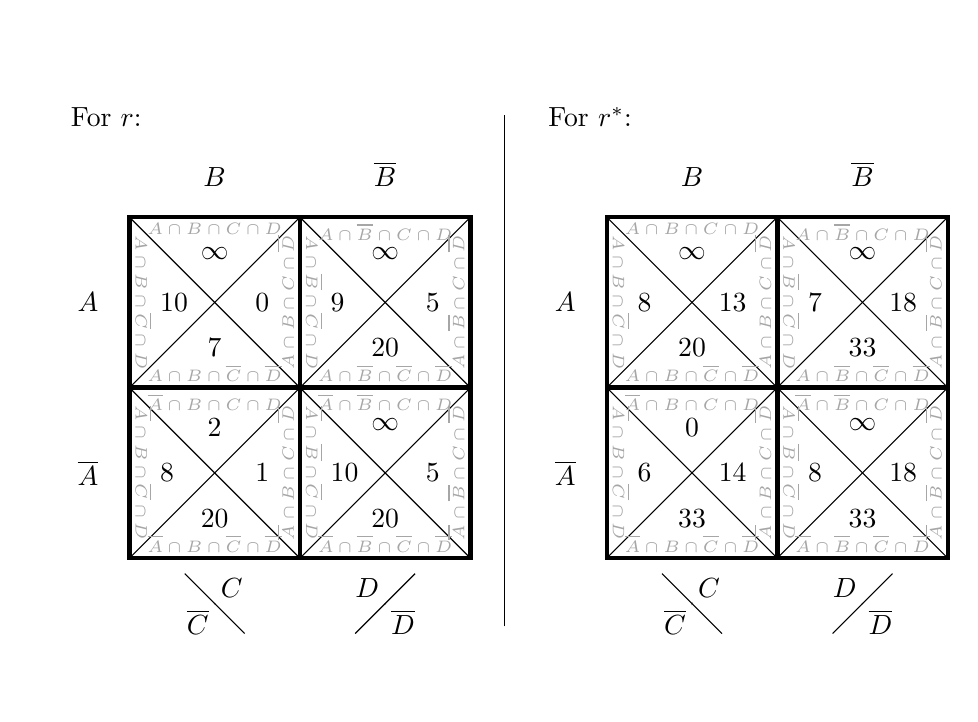
\begin{tikzpicture} [scale=\textwidth/14cm,
%appearances of inside recangle captions
sloped=false,
incaption/.style={color=gray, inner sep=0.05cm, font=\fontsize{6}{6}\sansmath\sffamily}]
\node at (-0.5,9) [draw=none,fill=none, above right] { };
\node at (-0.5,-0.5) [draw=none,fill=none, above right] { };

%BEGIN of grid for function "R"
\node at (0,8.25) [draw=none,fill=none,below right] {For $r$:};

%diagonal lines (thin):
\begin{scope} [thin]
	\draw (1,1.5)	-- (3.5,4);
	\draw (1,4)		-- (3.5,1.5);
	\draw (3.5,1.5) -- (6,4);
	\draw (3.5,4)	-- (6,1.5);
	\draw (1,4)		-- (3.5,6.5);
	\draw (1,6.5)	-- (3.5,4);
	\draw (3.5,4)	-- (6,6.5);
	\draw (3.5,6.5) -- (6,4);
\end{scope}

%rectangles (bold):
\begin{scope} [ultra thick]
	%rectangle 1 (lower left)
	\draw
	(1,1.5) --
	node[incaption, above=0cm] {$\overline{A}\cap B\cap\overline{C}\cap\overline{D}$}
	node[above=0.7em] {$20$}
	(3.5,1.5) --
	node[incaption, above=0cm, sloped] {$\overline{A}\cap B\cap C\cap\overline{D}$}
	node[left=0.7em] {$1$}
	(3.5,4)	--
	node[incaption, below=0cm] {$\overline{A}\cap B\cap C\cap D$}
	node[below=0.7em] {$2$}
	(1,4) --
	node[left=0.25cm] {$\overline{A}$}
	node[incaption, above=0cm, sloped] {$\overline{A}\cap B\cap\overline{C}\cap D$}
	node[right=0.7em] {$8$}
	(1,1.5) -- cycle;

	%rectangle 2 (lower right)
	\draw
	(3.5,1.5) --
	node[incaption, above=0cm] {$\overline{A}\cap\overline{B}\cap\overline{C}\cap\overline{D}$}
	node[above=0.7em] {$20$}
	(6,1.5)	--
	node[incaption, above=0cm, sloped] {$\overline{A}\cap\overline{B}\cap C\cap\overline{D}$}
	node[left=0.7em] {$5$}
	(6,4) --
	node[incaption, below=0cm] {$\overline{A}\cap\overline{B}\cap C\cap D$}
	node[below=0.7em] {$\infty$}
	(3.5,4)	--
	node[incaption, above=0cm, sloped] {$\overline{A}\cap\overline{B}\cap\overline{C}\cap D$}
	node[right=0.7em] {$10$}
	(3.5,1.5) -- cycle;

	%rectangle 3 (upper right)
	\draw (3.5,4) 	--
	node[incaption, above=0cm] {$A\cap\overline{B}\cap\overline{C}\cap\overline{D}$}
	node[above=0.7em] {$20$}
	(6,4) --
	node[incaption, above=0cm, sloped] {$A\cap\overline{B}\cap C\cap\overline{D}$}
	node[left=0.7em] {$5$}
	(6,6.5)	--
	node[above=0.25cm] {$\overline{B}$}
	node[incaption, below=0cm] {$A\cap\overline{B}\cap C\cap D$}
	node[below=0.7em] {$\infty$}
	(3.5,6.5) --
	node[incaption, above=0cm, sloped] {$A\cap\overline{B}\cap\overline{C}\cap D$}
	node[right=0.7em] {$9$}
	(3.5,4) --  cycle;

	%rectangle 4 (upper left)
	\draw (1,4)	--
	node[incaption, above=0cm] {$A\cap B\cap\overline{C}\cap\overline{D}$}
	node[above=0.7em] {$7$}
	(3.5,4)	--
	node[incaption, above=0cm, sloped] {$A\cap B\cap C\cap\overline{D}$}
	node[left=0.7em] {$0$}
	(3.5,6.5) --
	node[above=0.25cm] {$B$}
	node[incaption, below=0cm] {$A\cap B\cap C\cap D$}
	node[below=0.7em] {$\infty$}
	(1,6.5) --
	node[left=0.25cm] {$A$} node[incaption, sloped, above=0cm] {$A\cap B\cap\overline{C}\cap D$}
	node[right=0.7em] {$10$}
	(1,4) -- cycle;
\end{scope}

%captions below:
%for "C"/"not-C":
	\draw [color=gray,thin] (2.25cm-1.25em,1.5cm-2.5em-1.5ex)	-- (2.25cm+1.25em,1.5cm-1.5ex);
	\draw [thin] (2.25cm-1.25em,1.5cm-1.5ex) -- node[above right, fill=white, inner sep=2pt] {$C$} node[below left,fill=white, inner sep=2pt] {$\overline{C}$} (2.25cm+1.25em,1.5cm-2.5em-1.5ex);
%for "D"/"not-D":
	\draw [color=gray,thin] (4.75cm-1.25em,1.5cm-1.5ex) -- (4.75cm+1.25em,1.5cm-2.5em-1.5ex);
	\draw [thin] (4.75cm-1.25em,1.5cm-2.5em-1.5ex)	-- node[above left, fill=white, inner sep=2pt] {$D$} node[below right,fill=white, inner sep=2pt] {$\overline{D}$} (4.75cm+1.25em,1.5cm-1.5ex);

%END of grid for function "R"

%separating line
\draw (6.5,0.5) -- (6.5,8);



%BEGIN of grid for function "R*"
\begin{scope} [xshift=7cm]

\node at (0,8.25) [draw=none,fill=none,below right] {For $r^*$:};
%diagonal lines (thin):
\begin{scope} [thin]
	\draw (1,1.5)	-- (3.5,4);
	\draw (1,4)		-- (3.5,1.5);
	\draw (3.5,1.5) -- (6,4);
	\draw (3.5,4)	-- (6,1.5);
	\draw (1,4)		-- (3.5,6.5);
	\draw (1,6.5)	-- (3.5,4);
	\draw (3.5,4)	-- (6,6.5);
	\draw (3.5,6.5) -- (6,4);
\end{scope}

%rectangles (bold):
\begin{scope} [ultra thick]
	%rectangle 1 (lower left)
	\draw
	(1,1.5) --
	node[incaption, above=0cm] {$\overline{A}\cap B\cap\overline{C}\cap\overline{D}$}
	node[above=0.7em] {$33$}
	(3.5,1.5) --
	node[incaption, above=0cm, sloped] {$\overline{A}\cap B\cap C\cap\overline{D}$}
	node[left=0.7em] {$14$}
	(3.5,4)	--
	node[incaption, below=0cm] {$\overline{A}\cap B\cap C\cap D$}
	node[below=0.7em] {$0$}
	(1,4) --
	node[left=0.25cm] {$\overline{A}$}
	node[incaption, above=0cm, sloped] {$\overline{A}\cap B\cap\overline{C}\cap D$}
	node[right=0.7em] {$6$}
	(1,1.5) -- cycle;

	%rectangle 2 (lower right)
	\draw
	(3.5,1.5) --
	node[incaption, above=0cm] {$\overline{A}\cap\overline{B}\cap\overline{C}\cap\overline{D}$}
	node[above=0.7em] {$33$}
	(6,1.5)	--
	node[incaption, above=0cm, sloped] {$\overline{A}\cap\overline{B}\cap C\cap\overline{D}$}
	node[left=0.7em] {$18$}
	(6,4) --
	node[incaption, below=0cm] {$\overline{A}\cap\overline{B}\cap C\cap D$}
	node[below=0.7em] {$\infty$}
	(3.5,4)	--
	node[incaption, above=0cm, sloped] {$\overline{A}\cap\overline{B}\cap\overline{C}\cap D$}
	node[right=0.7em] {$8$}
	(3.5,1.5) -- cycle;

	%rectangle 3 (upper right)
	\draw (3.5,4) 	--
	node[incaption, above=0cm] {$A\cap\overline{B}\cap\overline{C}\cap\overline{D}$}
	node[above=0.7em] {$33$}
	(6,4) --
	node[incaption, above=0cm, sloped] {$A\cap\overline{B}\cap C\cap\overline{D}$}
	node[left=0.7em] {$18$}
	(6,6.5)	--
	node[above=0.25cm] {$\overline{B}$}
	node[incaption, below=0cm] {$A\cap\overline{B}\cap C\cap D$}
	node[below=0.7em] {$\infty$}
	(3.5,6.5) --
	node[incaption, above=0cm, sloped] {$A\cap\overline{B}\cap\overline{C}\cap D$}
	node[right=0.7em] {$7$}
	(3.5,4) --  cycle;

	%rectangle 4 (upper left)
	\draw (1,4)	--
	node[incaption, above=0cm] {$A\cap B\cap\overline{C}\cap\overline{D}$}
	node[above=0.7em] {$20$}
	(3.5,4)	--
	node[incaption, above=0cm, sloped] {$A\cap B\cap C\cap\overline{D}$}
	node[left=0.7em] {$13$}
	(3.5,6.5) --
	node[above=0.25cm] {$B$}
	node[incaption, below=0cm] {$A\cap B\cap C\cap D$}
	node[below=0.7em] {$\infty$}
	(1,6.5) --
	node[left=0.25cm] {$A$} node[incaption, sloped, above=0cm] {$A\cap B\cap\overline{C}\cap D$}
	node[right=0.7em] {$8$}
	(1,4) -- cycle;
\end{scope}

%captions below:
%for "C"/"not-C":
	\draw [color=gray,thin] (2.25cm-1.25em,1.5cm-2.5em-1.5ex)	-- (2.25cm+1.25em,1.5cm-1.5ex);
	\draw [thin] (2.25cm-1.25em,1.5cm-1.5ex) -- node[above right, fill=white, inner sep=2pt] {$C$} node[below left,fill=white, inner sep=2pt] {$\overline{C}$} (2.25cm+1.25em,1.5cm-2.5em-1.5ex);
%for "D"/"not-D":
	\draw [color=gray,thin] (4.75cm-1.25em,1.5cm-1.5ex) -- (4.75cm+1.25em,1.5cm-2.5em-1.5ex);
	\draw [thin] (4.75cm-1.25em,1.5cm-2.5em-1.5ex)	-- node[above left, fill=white, inner sep=2pt] {$D$} node[below right,fill=white, inner sep=2pt] {$\overline{D}$} (4.75cm+1.25em,1.5cm-1.5ex);

\end{scope}
%END of grid for function "R*"

\end{tikzpicture}
\caption{Sophia's old and new ranks for various conjunctions}
\label{huber:conjunctions1}
\end{figure}
% Here is where the first diagram ends
%\textcolor{blue}{A first picture will be inserted here that graphically represents the ranking function $R$ by showing how the various numbers are distributed over the relevant cells of the set of all possible worlds. A second picture will be inserted here that graphically represents how the ranking function $R^*$ arises from the ranking function $R$, and how the ranking function $R^{**}$ arises from the ranking function $R^*$. The following list of numbers will be deleted.}
%\begin{eqnarray*}
%R\left(A\cap B\cap C\cap D\right)&=&\infty\\
%R\left(A\cap B\cap C\cap\overline{D}\right)&=&0\\
%R\left(A\cap B\cap\overline{C}\cap D\right)&=&10\\
%R\left(A\cap B\cap\overline{C}\cap\overline{D}\right)&=&7\\
%R\left(A\cap\overline{B}\cap C\cap D\right)&=&\infty\\
%R\left(A\cap\overline{B}\cap C\cap\overline{D}\right)&=&5\\
%R\left(A\cap\overline{B}\cap\overline{C}\cap D\right)&=&9\\
%R\left(A\cap\overline{B}\cap\overline{C}\cap\overline{D}\right)&=&20\\
%R\left(\overline{A}\cap B\cap C\cap D\right)&=&2\\
%R\left(\overline{A}\cap B\cap C\cap\overline{D}\right)&=&1\\
%R\left(\overline{A}\cap B\cap\overline{C}\cap D\right)&=&8\\
%R\left(\overline{A}\cap B\cap\overline{C}\cap\overline{D}\right)&=&20\\
%R\left(\overline{A}\cap\overline{B}\cap C\cap D\right)&=&\infty\\
%R\left(\overline{A}\cap\overline{B}\cap C\cap\overline{D}\right)&=&5\\
%R\left(\overline{A}\cap\overline{B}\cap\overline{C}\cap D\right)&=&10\\
%R\left(\overline{A}\cap\overline{B}\cap\overline{C}\cap\overline{D}\right)&=&20
%\end{eqnarray*}
Then Sophia's new ranks are $r^*(\overline{C})=6$, $r^*(\overline{B})=7$, $r^*(A)=7$, $r^*(\overline{D})=13$.

Note that $C$ is a proposition Sophia believes both before and after revision by $D$, $r(\overline{C})>0$
and $r^*(\overline{C})>0,$ although $\overline{D}$ is positively relevant to, and so not independent of, $C$ in the sense that $r(\overline{C}\mid\overline{D})=7>6=r(\overline{C}\mid D).$ In other words, Sophia receives new information $D$ whose negation is positively relevant to, and so not independent of, her belief that $C$ without making her give up her belief that $C$. On the other hand, if Sophia considers $\overline{D}$ independent of a proposition $X$ before revision by $D$, %in the sense that $R\left(X\mid D\right)=R\left(X\mid\overline{D}\right)$ and $R\left(\overline{X}\mid D\right)=R\left(\overline{X}\mid\overline{D}\right)$,
then she also does so after revision by $D$. %in the sense that $R^*\left(X\mid D\right)=R^*\left(X\mid\overline{D}\right)$ and $R^*\left(\overline{X}\mid D\right)=R^*\left(\overline{X}\mid\overline{D}\right)$
More generally, suppose two propositions $A$ and $B$ are independent according to a ranking function $r$,
$r(A\mid B)=r(A\mid\overline{B})$ and $r(\overline{A}\mid B)=r(\overline{A}\mid\overline{B})$. In this case $A$ and $B$ are independent according to any ranking function $r^*$ that results from $r$ by what we may call a ``Spohn shift'' on the partition $\{B,\overline{B}\}$, i.e. the result of Spohn conditionalization on this partition for an arbitrary pair of natural numbers.

This feature, which is known as \emph{rigidity}, vindicates the idea behind \citet{jt07}'s proposal that revision should preserve independencies. It does so by fixing their notion of independence. For more on the definition of rank-theoretic independence see \citet{s99}. As an aside let me note that, while rigidity is generally considered to be a desirable feature of an update rule, \citet{w09, w15} uses rigidity to argue that neither Bayesianism nor Dempster-Shafer theory \citep{h09} nor ranking theory can handle a phenomenon he terms \emph{perceptual undermining}. \citet{h14a} defends these theories against Weisberg's charge.

Spohn conditionalization gives Sophia a complete new ranking function $r^*$ that she can use to revise her newly acquired belief set
$$\begin{cal}B\end{cal}^*=\left\{X\in\begin{cal}A\end{cal}: r^*\left(\overline{X}\right)>0\right\}$$
a second time when she learns on Tuesday that it is sunny after all. All she has to do is tell us how strongly she then disbelieves the proposition $B$ that it will rain on Tuesday. If $r^{**}\left(B\right)=13$, her newer ranks are $r^{**}(\overline{A})=1$, $r^{**}(C)=11$, $r^{**}(\overline{D})=11$. See \autoref{huber:conjunctions2}.

% HERE IS WHERE THE SECOND DIAGRAM BEGINS
\begin{figure}[ht]
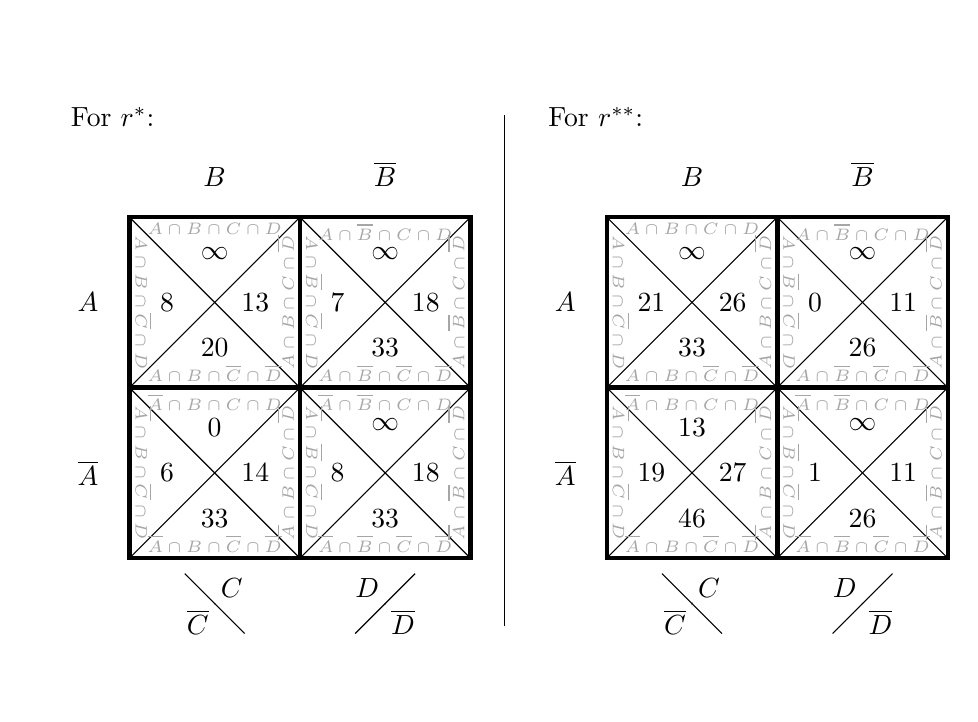
\begin{tikzpicture} [scale=\textwidth/14cm,
%appearances of inside recangle captions
sloped=false,
incaption/.style={color=gray, inner sep=0.05cm, font=\fontsize{6}{6}\sansmath\sffamily}]

\node at (-0.5,9) [draw=none,fill=none, above right] { };
\node at (-0.5,-0.5) [draw=none,fill=none, above right] { };

%BEGIN of grid for function "R*"
\node at (0,8.25) [draw=none,fill=none,below right] {For $r^*$:};

%diagonal lines (thin):
\begin{scope} [thin]
	\draw (1,1.5)	-- (3.5,4);
	\draw (1,4)		-- (3.5,1.5);
	\draw (3.5,1.5) -- (6,4);
	\draw (3.5,4)	-- (6,1.5);
	\draw (1,4)		-- (3.5,6.5);
	\draw (1,6.5)	-- (3.5,4);
	\draw (3.5,4)	-- (6,6.5);
	\draw (3.5,6.5) -- (6,4);
\end{scope}

%rectangles (bold):
\begin{scope} [ultra thick]
	%rectangle 1 (lower left)
	\draw
	(1,1.5) --
	node[incaption, above=0cm] {$\overline{A}\cap B\cap\overline{C}\cap\overline{D}$}
	node[above=0.7em] {$33$}
	(3.5,1.5) --
	node[incaption, above=0cm, sloped] {$\overline{A}\cap B\cap C\cap\overline{D}$}
	node[left=0.7em] {$14$}
	(3.5,4)	--
	node[incaption, below=0cm] {$\overline{A}\cap B\cap C\cap D$}
	node[below=0.7em] {$0$}
	(1,4) --
	node[left=0.25cm] {$\overline{A}$}
	node[incaption, above=0cm, sloped] {$\overline{A}\cap B\cap\overline{C}\cap D$}
	node[right=0.7em] {$6$}
	(1,1.5) -- cycle;

	%rectangle 2 (lower right)
	\draw
	(3.5,1.5) --
	node[incaption, above=0cm] {$\overline{A}\cap\overline{B}\cap\overline{C}\cap\overline{D}$}
	node[above=0.7em] {$33$}
	(6,1.5)	--
	node[incaption, above=0cm, sloped] {$\overline{A}\cap\overline{B}\cap C\cap\overline{D}$}
	node[left=0.7em] {$18$}
	(6,4) --
	node[incaption, below=0cm] {$\overline{A}\cap\overline{B}\cap C\cap D$}
	node[below=0.7em] {$\infty$}
	(3.5,4)	--
	node[incaption, above=0cm, sloped] {$\overline{A}\cap\overline{B}\cap\overline{C}\cap D$}
	node[right=0.7em] {$8$}
	(3.5,1.5) -- cycle;

	%rectangle 3 (upper right)
	\draw (3.5,4) 	--
	node[incaption, above=0cm] {$A\cap\overline{B}\cap\overline{C}\cap\overline{D}$}
	node[above=0.7em] {$33$}
	(6,4) --
	node[incaption, above=0cm, sloped] {$A\cap\overline{B}\cap C\cap\overline{D}$}
	node[left=0.7em] {$18$}
	(6,6.5)	--
	node[above=0.25cm] {$\overline{B}$}
	node[incaption, below=0cm] {$A\cap\overline{B}\cap C\cap D$}
	node[below=0.7em] {$\infty$}
	(3.5,6.5) --
	node[incaption, above=0cm, sloped] {$A\cap\overline{B}\cap\overline{C}\cap D$}
	node[right=0.7em] {$7$}
	(3.5,4) --  cycle;

	%rectangle 4 (upper left)
	\draw (1,4)	--
	node[incaption, above=0cm] {$A\cap B\cap\overline{C}\cap\overline{D}$}
	node[above=0.7em] {$20$}
	(3.5,4)	--
	node[incaption, above=0cm, sloped] {$A\cap B\cap C\cap\overline{D}$}
	node[left=0.7em] {$13$}
	(3.5,6.5) --
	node[above=0.25cm] {$B$}
	node[incaption, below=0cm] {$A\cap B\cap C\cap D$}
	node[below=0.7em] {$\infty$}
	(1,6.5) --
	node[left=0.25cm] {$A$} node[incaption, sloped, above=0cm] {$A\cap B\cap\overline{C}\cap D$}
	node[right=0.7em] {$8$}
	(1,4) -- cycle;
\end{scope}

%captions below:
%for "C"/"not-C":
	\draw [color=gray,thin] (2.25cm-1.25em,1.5cm-2.5em-1.5ex)	-- (2.25cm+1.25em,1.5cm-1.5ex);
	\draw [thin] (2.25cm-1.25em,1.5cm-1.5ex) -- node[above right, fill=white, inner sep=2pt] {$C$} node[below left,fill=white, inner sep=2pt] {$\overline{C}$} (2.25cm+1.25em,1.5cm-2.5em-1.5ex);
%for "D"/"not-D":
	\draw [color=gray,thin] (4.75cm-1.25em,1.5cm-1.5ex) -- (4.75cm+1.25em,1.5cm-2.5em-1.5ex);
	\draw [thin] (4.75cm-1.25em,1.5cm-2.5em-1.5ex)	-- node[above left, fill=white, inner sep=2pt] {$D$} node[below right,fill=white, inner sep=2pt] {$\overline{D}$} (4.75cm+1.25em,1.5cm-1.5ex);

%END of grid for function "R*"

%separating line
\draw (6.5,0.5) -- (6.5,8);



%BEGIN of grid for function "R**"
\begin{scope} [xshift=7cm]

\node at (0,8.25) [draw=none,fill=none,below right] {For $r^{**}$:};
%diagonal lines (thin):
\begin{scope} [thin]
	\draw (1,1.5)	-- (3.5,4);
	\draw (1,4)		-- (3.5,1.5);
	\draw (3.5,1.5) -- (6,4);
	\draw (3.5,4)	-- (6,1.5);
	\draw (1,4)		-- (3.5,6.5);
	\draw (1,6.5)	-- (3.5,4);
	\draw (3.5,4)	-- (6,6.5);
	\draw (3.5,6.5) -- (6,4);
\end{scope}

%rectangles (bold):
\begin{scope} [ultra thick]
	%rectangle 1 (lower left)
	\draw
	(1,1.5) --
	node[incaption, above=0cm] {$\overline{A}\cap B\cap\overline{C}\cap\overline{D}$}
	node[above=0.7em] {$46$}
	(3.5,1.5) --
	node[incaption, above=0cm, sloped] {$\overline{A}\cap B\cap C\cap\overline{D}$}
	node[left=0.7em] {$27$}
	(3.5,4)	--
	node[incaption, below=0cm] {$\overline{A}\cap B\cap C\cap D$}
	node[below=0.7em] {$13$}
	(1,4) --
	node[left=0.25cm] {$\overline{A}$}
	node[incaption, above=0cm, sloped] {$\overline{A}\cap B\cap\overline{C}\cap D$}
	node[right=0.7em] {$19$}
	(1,1.5) -- cycle;

	%rectangle 2 (lower right)
	\draw
	(3.5,1.5) --
	node[incaption, above=0cm] {$\overline{A}\cap\overline{B}\cap\overline{C}\cap\overline{D}$}
	node[above=0.7em] {$26$}
	(6,1.5)	--
	node[incaption, above=0cm, sloped] {$\overline{A}\cap\overline{B}\cap C\cap\overline{D}$}
	node[left=0.7em] {$11$}
	(6,4) --
	node[incaption, below=0cm] {$\overline{A}\cap\overline{B}\cap C\cap D$}
	node[below=0.7em] {$\infty$}
	(3.5,4)	--
	node[incaption, above=0cm, sloped] {$\overline{A}\cap\overline{B}\cap\overline{C}\cap D$}
	node[right=0.7em] {$1$}
	(3.5,1.5) -- cycle;

	%rectangle 3 (upper right)
	\draw (3.5,4) 	--
	node[incaption, above=0cm] {$A\cap\overline{B}\cap\overline{C}\cap\overline{D}$}
	node[above=0.7em] {$26$}
	(6,4) --
	node[incaption, above=0cm, sloped] {$A\cap\overline{B}\cap C\cap\overline{D}$}
	node[left=0.7em] {$11$}
	(6,6.5)	--
	node[above=0.25cm] {$\overline{B}$}
	node[incaption, below=0cm] {$A\cap\overline{B}\cap C\cap D$}
	node[below=0.7em] {$\infty$}
	(3.5,6.5) --
	node[incaption, above=0cm, sloped] {$A\cap\overline{B}\cap\overline{C}\cap D$}
	node[right=0.7em] {$0$}
	(3.5,4) --  cycle;

	%rectangle 4 (upper left)
	\draw (1,4)	--
	node[incaption, above=0cm] {$A\cap B\cap\overline{C}\cap\overline{D}$}
	node[above=0.7em] {$33$}
	(3.5,4)	--
	node[incaption, above=0cm, sloped] {$A\cap B\cap C\cap\overline{D}$}
	node[left=0.7em] {$26$}
	(3.5,6.5) --
	node[above=0.25cm] {$B$}
	node[incaption, below=0cm] {$A\cap B\cap C\cap D$}
	node[below=0.7em] {$\infty$}
	(1,6.5) --
	node[left=0.25cm] {$A$} node[incaption, sloped, above=0cm] {$A\cap B\cap\overline{C}\cap D$}
	node[right=0.7em] {$21$}
	(1,4) -- cycle;
\end{scope}

%captions below:
%for "C"/"not-C":
	\draw [color=gray,thin] (2.25cm-1.25em,1.5cm-2.5em-1.5ex)	-- (2.25cm+1.25em,1.5cm-1.5ex);
	\draw [thin] (2.25cm-1.25em,1.5cm-1.5ex) -- node[above right, fill=white, inner sep=2pt] {$C$} node[below left,fill=white, inner sep=2pt] {$\overline{C}$} (2.25cm+1.25em,1.5cm-2.5em-1.5ex);
%for "D"/"not-D":
	\draw [color=gray,thin] (4.75cm-1.25em,1.5cm-1.5ex) -- (4.75cm+1.25em,1.5cm-2.5em-1.5ex);
	\draw [thin] (4.75cm-1.25em,1.5cm-2.5em-1.5ex)	-- node[above left, fill=white, inner sep=2pt] {$D$} node[below right,fill=white, inner sep=2pt] {$\overline{D}$} (4.75cm+1.25em,1.5cm-1.5ex);

\end{scope}
%END of grid for function "R**"


\end{tikzpicture}
\caption{Sophia's new and newer ranks for various conjunctions}
\label{huber:conjunctions2}
\end{figure}
% Here is where the second diagram ends

This means that Sophia did not mishear the weather forecast, but was too gullible (or so we assume for purposes of illustration), and so has to give up her belief $C$ that weather forecasts are always right. In addition she also has to regain her belief $A$ that it will be sunny on Wednesday.

At the end of this section Sophia's doxastic career is pictured as a sequence of ``onions.'' The difference to the AGM theory is that, in ranking theory, the layers carry numbers which reflect how far apart they are from each other according to the ideal agent's doxastic state. A different way to picture the situation is to allow for \emph{empty} layers and to have one, possibly empty, layer for each natural number.

We see that ranking theory handles indefinitely iterated belief revisions. It does so in contrast to the AGM theory of belief revision. However, it does so also in contrast to probability theory. As yet another aside, let me briefly explain why. In probability theory the ideal doxastic agent is sometimes forced to assign probability $0$ to some non-empty or consistent proposition. In order to enable her to learn such propositions the ideal doxastic agent is usually represented by a Popper-R\'{e}nyi measure which is more general than a classical probability (\citealp{p55, r55, s70, s86}; Easwaran, \citethisvolume{thisvolume:easwaran}). However, as already noted by \citet{h76a}, Popper-R\'{e}nyi measures violate the principal of categorical matching and so cannot handle iterated revisions of degrees of belief: the result of conditionalizing a Popper-R\'{e}nyi measure is not another Popper-R\'{e}nyi measure, but a classical probability; and as \citet{b95} notes, there is no straightforward analogue of Jeffrey conditionalization for Popper-R\'{e}nyi measures. \citet{s06a} provides an even more general notion of probability, \emph{ranked probability}, which results from making probabilities the objects of rank-theoretic belief. It handles iterated revisions of probabilistic degrees of belief and satisfies the principal of categorical matching: the result of conditionalizing a ranked probability is another ranked probability.

Ranking theory is a normative theory that addresses the question how an ideal doxastic agent should organize her beliefs and conditional beliefs at a given moment in time, and how she should revise these beliefs across time if she receives new information of various formats. Why should an ideal doxastic agent obey the norms of ranking theory? That is, why should an ideal doxastic agent organize her beliefs and conditional beliefs at a given moment in time according to axioms (\ref{rank1})--(\ref{rank3})? And why should she update her beliefs and conditional beliefs across time according to update rules (\ref{rankrule1})--(\ref{rankrule3}) if she receives new information of the appropriate format? Who are we, Sophia asks, to tell her what---or rather: how---to believe? To answer these questions, and to respond to Sophia, we need a bit of terminology.

An ideal doxastic agent's \emph{grade of entrenchment} for a proposition $A$ is defined as the smallest number $n$ such that she would give up her disbelief in $A$ if she received the information $A$ from $n$ sources she deemed independent and minimally positively reliable, \textit{mp-reliable}, about $A$, and this was all that directly affected her doxastic state. If the ideal doxastic agent does not disbelieve $A$ to begin with, her grade of entrenchment for $A$ is $0$. Her grade of entrenchment for $A$ is higher, the more information sources of the sort described it would take for her to give up her disbelief in $A$.

As mentioned previously, whereas probabilities are measured on an absolute scale, ranks are at best measured on a ratio scale. The same is true for grades of entrenchment. Therefore we need to fix a \emph{unit} for these grades of entrenchment. We need to do the same when we want to report the amount of money in your bank account, which is measured on a ratio scale, or the temperature in Vienna on January 1, 2018, which is measured on an interval scale. To say that the amount of money in your bank account, or the temperature in Vienna on January 1, 2018, equals $17$ is not saying anything if we do not also specify a unit such as Euros or degrees of Celsius. Information sources that are deemed mp-reliable are used to define the unit in which grades of entrenchment are reported. Furthermore, to guarantee that these units can be added and compared, just as we can add and compare sums of Euros and degrees of Celsius, we need to make sure that these information sources are not only deemed to be mp-reliable by the ideal doxastic agent, but also independent in the relevant sense.

%Information sources that are deemed independent and mp-reliable are defined in terms of grades of disbelief. The same is true of grades of entrenchment, which go hand in hand with grades of disbelief. %For as we will see momentarily, to the extent that subjective grades of disbelief should obey the static and dynamic norms of ranking theory, they should do so, because they correspond one-to-one to grades of entrenchment, and because the latter should satisfy the static and dynamic norms of ranking theory.
%This contrasts with the otherwise similar relationship in Bayesianism between an ideal doxastic agent's degrees of belief, or subjective probabilities, and the betting ratios she deems to be fair. The betting ratios she deems to be fair can sometimes be used to measure her subjective degrees of belief, but not to define them \citep{eh07}. %Bay is Sophia's friend. Bay's fair betting ratios are not always independent of the truth values of the propositions she is imagined to bet on, nor are they never affected by the stakes at issue.
%In Bayesianism there is a gap between fair betting ratios and subjective degrees of belief, because there is a gap between believing a proposition to a certain degree, and acting on this degree of belief. This is different in the present case, where grades of belief are merely linked to the potential revision of those very beliefs they are grades of.

We non-ideal doxastic agents generally do not deem our sources of information independent or mp-reliable. One expert's saying $A$ will sometimes make us stop disbelieving $A$ immediately, while the sermons of a dozen others won't. And the last-born's telling a parent that there is no red wine left after the first-born has already confessed to drinking it up won't make much of a difference to the parent's grade of disbelief that there is red wine left. However, this is no argument against the usefulness of this notion. Information sources that are deemed independent and mp-reliable are a theoretical construct that are assumed or postulated to exist. They are the smallest units such that the reliability one deems any possible information source to possess can be expressed as a multiple of them.

%our ideal doxastic agent is ideal, and so is able to access all of her beliefs and conditional beliefs as well as able to identify which shifts in strength of belief are minimal. % as well as able to determine if two shifts in strength of belief are identical.
%Given these assumptions there is a one-to-one correspondence between the ideal doxastic agent's grades of disbelief, or subjective ranks, and her grades of entrenchment. The latter are defined in terms of the former and various counterfactual conditionals, because \emph{in fact} she may never encounter the information sources that she deems to be independent and mp-reliable.% (this raises a circularity concern that I will address in chapter 10).%: her grade of entrenchment for a proposition $A$ is defined as the smallest number $n$ such that she would give up her disbelief in $A$ if she received the information $A$ from $n$ sources that she deemed independent and minimally positively reliable about $A$.


%Independent and minimally positively reliable information sources for a proposition are idealized entities that are used to define the ideal doxastic agent's degrees of entrenchment. Information sources as we know them -- friends, newspapers, search engines -- are neither independent nor minimally positively reliable. One person's saying $A$ will sometimes make somebody stop disbelieving $A$ immediately, while the sermons of a dozen of others won't. Sophia's son telling her that $A$ after her daughter has already explained to her why $A$ won't make much of a difference to Sophia. However, apart from this idealization, the agent's degrees of entrenchment are observable, provided she is honest. In contrast to this, the agent's grades of disbelief, her ranks, are theoretical entities.

%The relation between the ideal doxastic agent's grades of disbelief and her degrees of entrenchment is a delicate one. Minimally degrees of entrenchment are used to measure grades of disbelief; maximally the latter can be defined in terms of the former. (One possibility may be to define the ideal doxastic agent's subjective rank for a proposition $A$ as the number of information sources saying $A$ that it would take for her to give up her belief in $A$, if those information sources were independent and minimally positively reliable.) The situation is similar in Bayesianism with its notion of the ideal doxastic agent's \emph{betting ratio}, or \emph{fair betting ratio}. Minimally, (fair) betting ratios are used to measure subjective probabilities; maximally the former are used to define the latter (see Eriksson \& H�jek 2007). Bay is Sophia's friend. Bay's (fair) betting ratios are not always independent of the truth values of the propositions she is forced to bet on, nor are they never affected by the stakes at issue. This does not mean that the notion of a (fair) betting ratio needs to be discarded.

Let $\varrho$ be the ideal doxastic agent's entrenchment function, i.e. the function that summarizes her grades of entrenchment for all propositions from $\cal A$. Her \emph{belief set} $\begin{cal}B\end{cal}_\varrho$ is the set of propositions with a positive grade of entrenchment,
$$\begin{cal}B\end{cal}_\varrho=\left\{A\in\begin{cal}A\end{cal}:\varrho\left(\overline{A}\right)>0\right\}.$$
Her belief set conditional on the consistent proposition $C$ is the set of propositions with a positive grade of entrenchment conditional on $C$,
$$\begin{cal}B\end{cal}_{\varrho\left(\cdot\mid C\right)}=\left\{A\in\begin{cal}A\end{cal}:\varrho\left(\overline{A}\mid C\right)>0\right\}.$$ % so that $\begin{cal}B\end{cal}_{\varrho\left(\cdot\mid W\right)}=\begin{cal}B\end{cal}_\varrho$.
%Note that these (conditional) belief sets are defined in terms of the ideal doxastic agent's (conditional) grades of entrenchment, not her (conditional) grades of disbelief, her (conditional) subjective ranks.
$\begin{cal}B\end{cal}\subseteq\begin{cal}A\end{cal}$ is \emph{consistent in the finite\,/\,countable\,/\,complete sense} if, and only if, for every finite/countable/arbitrary $\begin{cal}B\end{cal}^-\subseteq\begin{cal}B\end{cal}$, $\bigcap\begin{cal}B\end{cal}^-\neq\emptyset$. It is \emph{deductively closed in the finite\,/\,countable\,/\,complete sense} if, and only if, for every finite/countable/arbitrary $\begin{cal}B\end{cal}^-\subseteq\begin{cal}B\end{cal}$ and all $A\in\begin{cal}A\end{cal}$: if $\bigcap\begin{cal}B\end{cal}^-\subseteq A$, then $A\in\begin{cal}B\end{cal}$. Similarly, for a proposition $C$ from $\cal A$, $\begin{cal}B\end{cal}\subseteq\begin{cal}A\end{cal}$ is \emph{conditionally consistent given $C$ in the finite\,/\,countable\,/\,complete sense} if, and only if, for every finite/countable/arbitrary $\begin{cal}B\end{cal}^-\subseteq\begin{cal}B\end{cal}$: $C\cap\bigcap\begin{cal}B\end{cal}^-\neq\emptyset$. It is \emph{conditionally deductively closed given $C$ in the finite\,/\,countable\,/\,complete sense} if, and only if, for every finite/countable/arbitrary $\begin{cal}B\end{cal}^-\subseteq\begin{cal}B\end{cal}$ and all $A\in\begin{cal}A\end{cal}$: if $C\cap\bigcap\begin{cal}B\end{cal}^-\subseteq A$, then $A\in\begin{cal}B\end{cal}$.


%A (conditional) belief set $\begin{cal}B\end{cal}\subseteq\begin{cal}A\end{cal}$ is \emph{consistent in the finite / countable / complete sense} if, and only if, for every finite / countable / arbitrary set of propositions $\begin{cal}B\end{cal}^-\subseteq\begin{cal}B\end{cal}$: $\bigcap\begin{cal}B\end{cal}^-\neq\emptyset$. A (conditional) belief set $\begin{cal}B\end{cal}\subseteq\begin{cal}A\end{cal}$ is \emph{deductively closed in the finite / countable / complete sense} if, and only if, for every finite / countable / arbitrary set of propositions $\begin{cal}B\end{cal}^-\subseteq\begin{cal}B\end{cal}$ and all propositions $A\in\begin{cal}A\end{cal}$: if $\bigcap\begin{cal}B\end{cal}^-\subseteq A$, then $A\in\begin{cal}B\end{cal}$.

%Let $\varrho$ be the ideal doxastic agent's entrenchment function, i.e. the function that summarizes her grades of entrenchment for all propositions under consideration. Then her \emph{belief set} $\begin{cal}B\end{cal}_\varrho$ is defined as the set of propositions whose negations have a positive grade of entrenchment, $\begin{cal}B\end{cal}_\varrho=\left\{A\in\begin{cal}A\end{cal}:\varrho\left(\overline{A}\right)>0\right\}$. The ideal doxastic agent's belief set $\begin{cal}B\end{cal}_\varrho\subseteq\begin{cal}A\end{cal}$ is \emph{consistent in the finite / countable / complete sense} if, and only if, for every finite / countable / arbitrary set of propositions $\begin{cal}B\end{cal}\subseteq\begin{cal}B\end{cal}_\varrho$: $\bigcap\cal B\neq\emptyset$. Her belief set $\begin{cal}B\end{cal}\subseteq\begin{cal}A\end{cal}$ is \emph{deductively closed in the finite / countable / complete sense} if, and only if, for every finite / countable / arbitrary set of propositions $\begin{cal}B\end{cal}\subseteq\begin{cal}B\end{cal}_\varrho$ and all propositions $A$ from $\begin{cal}A\end{cal}$: if $\bigcap\begin{cal}B\end{cal}\subseteq A$, then $A\in\begin{cal}B\end{cal}_\varrho$.

Now we can respond to Sophia as well as answer the question why an ideal doxastic agent should organize her beliefs and conditional beliefs at a given moment in time according to axioms (\ref{rank1})--(\ref{rank3}), and why she should update her beliefs and conditional beliefs across time according to update rules (\ref{rankrule1})--(\ref{rankrule3}) if she receives new information of the appropriate format. She should do so, because
\begin{theorem}
An ideal doxastic agent's belief set $\begin{cal}B\end{cal}_\varrho$ and conditional belief sets $\begin{cal}B\end{cal}_{\varrho\left(\cdot\mid C\right)}$ for consistent conditions $C$ are (conditionally) consistent and deductively closed in the finite / countable / complete sense (given $C$)---and would remain so in response to any finite sequence of experiences---if, and only if, $\varrho$ is a finitely / countably / completely minimitive ranking function that would be revised according to update rules (\ref{rankrule1})--(\ref{rankrule3}).% Grades of entrenchment are assumed to be numbers from $\mathbb{N}\cup\left{\infty\right)$.
\end{theorem}
This theorem from \citet{h07} rests on several unstated assumptions which are spelled out in \citet{h19}.

The argument based on this theorem is supposed to establish the thesis that an ideal doxastic agent's beliefs and conditional beliefs should obey the synchronic and diachronic rules of ranking theory. It provides a means-end justification for this thesis in the spirit of epistemic consequentialism \citep{p02, s02a}. The idea is that obeying the normative constraints of ranking theory is a (necessary and sufficient) means to attaining the end of being ``eternally consistent and deductively closed.'' The latter end in turn is a (necessary, but insufficient) means to attaining the end of always having only true beliefs, and, subject to the constraint that \emph{all} of them are true, as many thereof as possible. To the extent that the ideal doxastic agent has this end, she should obey the norms of ranking theory. It is not that we are telling Sophia what and how to believe. \emph{She} is the one who is assumed to have these ends. We merely point out the obtaining means-end relationship. Of course, if Sophia does not desire to always hold only true beliefs, and, subject to the constraint that all of them are true, as many thereof as possible, our response will cut no ice. But that is beside the point: it is mistaking a hypothetical imperative for a categorical imperative.

\citet{beh} discuss the implications of this result as well as its Bayesian role-model, Joyce's (\citeyearhyper{j98}, \citeyearhyper{j09}) ``non-pragmatic vindication of probabilism'' (see also \citealt{p11,p13}), for considering doxastic rationality a form of instrumental rationality, and for means-end epistemology in general. Alternatively one may use the representation result by \citet{hs08}, or the rank-theoretic decision theory by \citet{gs00}, to obtain a justification of ranking theory that is deontological in spirit. For instance, the former result can be used to argue that all and only ranking functions obey the duties, or categorical imperatives, of iterated belief contraction, where these duties, or categorical imperatives, take the form of axioms for iterated contractions of beliefs.

\autoref{huber:onion1} depicts Sophia's ranking functions $r$ and $r^*$ as ``numbered onions.'' Alternatively (\autoref{huber:onion2}) Sophia's ranking function $r$ can be pictured as an onion with one, possibly empty, layer $r^{-1}\left(n\right)$ for each natural number $n$. Sophia's old rank for $D$ is $2$, i.e. $r(D)=2$, and her old rank for $\overline{D}$ is $0$, i.e. $r(\overline{D})=0$. Sophia's new ranking function $r^*$ results from her old ranking function $r$ by first improving the possible worlds in which $D$ is true by $2$ ranks so that the new rank of $D$ is $0$, i.e. $r^*\left(D\right)=0$. In a second step the possible worlds in which $\overline{D}$ is true are deteriorated by $13$ ranks so that the new rank of $\overline{D}$ is $13$, i.e. $r^*(\overline{D})=13$. The relative positions of the possible worlds in which $D$ is true, and the possible worlds in which $\overline{D}$ is true, are expressed in the conditional ranking functions $r(\cdot\mid D)=r^*(\cdot\mid D)$ and $r(\cdot\mid\overline{D})=r^*(\cdot\mid\overline{D})$. These relative positions or conditional ranks are kept fixed.

% HERE IS WHERE THE FIRST ONION BEGINS
\begin{figure}
\begin{tikzpicture} [scale=\textwidth/14cm] %appearances of inside circle captions


\definecolor{gray}{gray}{0.65};
\definecolor{lightgray}{gray}{0.80};
\definecolor{darkgray}{gray}{0.55};

% these coordinates guarantee the graph's total size
\node at (-6,5.5) [draw=none,fill=none, above right] { };

% paints the background for the "new information"
\fill[lightgray] (5.5,5.2) arc (90:270:5.5 and 5.2);

%first, the spheres' backgrounds are filled according to "R"
\fill [fill=gray] (0,0) circle (5.0);
\fill [fill=white](0,0) circle (4.5);
\fill [fill=gray] (0,0) circle (4.0);
\fill [fill=gray] (0,0) circle (3.5);
\fill [fill=gray] (0,0) circle (3.0);
\fill [fill=white](0,0) circle (2.5);
\fill [fill=white](0,0) circle (2.0);
\fill [fill=gray] (0,0) circle (1.5);
\fill [fill=white](0,0) circle (1.0);
\fill [fill=white](0,0) circle (0.5);

%then, the spheres' backgrounds according to "R*" are layed over the "R"-backgrounds
\begin{scope}
\clip (0,0) circle (5.0);
\fill[darkgray] (5.5,5.2) arc (90:270:5.5 and 5.2);
\end{scope}
\begin{scope}
\clip (0,0) circle (4.5);
\fill[lightgray] (5.5,5.2) arc (90:270:5.5 and 5.2);
\end{scope}
\begin{scope}
\clip (0,0) circle (4.0);
\fill[darkgray] (5.5,5.2) arc (90:270:5.5 and 5.2);
\end{scope}
\begin{scope}
\clip (0,0) circle (3.5);
\fill[darkgray] (5.5,5.2) arc (90:270:5.5 and 5.2);
\end{scope}
\begin{scope}
\clip (0,0) circle (3.0);
\fill[darkgray] (5.5,5.2) arc (90:270:5.5 and 5.2);
\end{scope}
\begin{scope}
\clip (0,0) circle (2.5);
\fill[lightgray] (5.5,5.2) arc (90:270:5.5 and 5.2);
\end{scope}
\begin{scope}
\clip (0,0) circle (2.0);
\fill[lightgray] (5.5,5.2) arc (90:270:5.5 and 5.2);
\end{scope}
\begin{scope}
\clip (0,0) circle (1.5);
\fill[darkgray] (5.5,5.2) arc (90:270:5.5 and 5.2);
\end{scope}
\begin{scope}
\clip (0,0) circle (1.0);
\fill[lightgray] (5.5,5.2) arc (90:270:5.5 and 5.2);
\end{scope}
\begin{scope}
\clip (0,0) circle (0.5);
\fill[lightgray] (5.5,5.2) arc (90:270:5.5 and 5.2);
\end{scope}



%spheres from outer to inner
\begin{scope} [thick]
\draw (0,0) circle (5.0) node at ($(0,0)+(260:5.0)$) [above=-0.05cm] {$\infty$}
                         node at ($(0,0)+(0:5.0)$)   [left=-0.1cm]  {$\infty$}
                         node at ($(0,0)+(135:5.0)$) [below right=-0.1cm] {$D$};
\draw (0,0) circle (4.5) node at ($(0,0)+(260:4.5)$) [above=-0.05cm] {20}
                         node at ($(0,0)+(0:4.5)$)   [left=-0.1cm]  {33};
\draw (0,0) circle (4.0) node at ($(0,0)+(260:4.0)$) [above=-0.05cm] {10}
                         node at ($(0,0)+(0:4.0)$)   [left]  {8}
                         node at ($(0,0)+(135:4.0)$) [below right=-0.1cm] {$D$};
\draw (0,0) circle (3.5) node at ($(0,0)+(260:3.5)$) [above=-0.05cm] {9}
                         node at ($(0,0)+(0:3.5)$)   [left]  {7}
                         node at ($(0,0)+(135:3.5)$) [below right=-0.1cm] {$D$};
\draw (0,0) circle (3.0) node at ($(0,0)+(260:3.0)$) [above=-0.05cm] {8}
                         node at ($(0,0)+(0:3.0)$)   [left]  {6}
                         node at ($(0,0)+(135:3.0)$) [below right=-0.1cm] {$D$};
\draw (0,0) circle (2.5) node at ($(0,0)+(260:2.5)$) [above=-0.05cm] {7}
                         node at ($(0,0)+(0:2.5)$)   [left=-0.1cm]  {20};
\draw (0,0) circle (2.0) node at ($(0,0)+(260:2.0)$) [above=-0.05cm] {5}
                         node at ($(0,0)+(0:2.0)$)   [left=-0.1cm]  {18};
\draw (0,0) circle (1.5) node at ($(0,0)+(260:1.5)$) [above=-0.05cm] {2}
                         node at ($(0,0)+(0:1.5)$)   [left]  {0}
                         node at ($(0,0)+(135:1.5)$) [below right=-0.1cm] {$D$};
\draw (0,0) circle (1.0) node at ($(0,0)+(260:1.0)$) [above=-0.05cm] {1}
                         node at ($(0,0)+(0:1.0)$)   [left=-0.1cm]  {14};
\draw (0,0) circle (0.5) node [left] {0}
                         node [right=-0.1cm] {13};
\end{scope}

%new information: "R^* (D) = 13"
\begin{scope} [ultra thick]
\draw (5.5,5.2) node [right] {$r^* (D) = 13$} arc (90:270:5.5 and 5.2);
\end{scope}

%labels "R" and "R*"
\begin{scope}
% \node [font=\fontsize{14}{16.8}] at (-4.5,-4.5) {$r$};
% \node [font=\fontsize{14}{16.8}] at (4.75,4.5)   {$r^*$};
\node at (-4.5,-4.5) {\Large $r$};
\node at (4.75,4.5)  {\Large $r^*$};
\end{scope}]

\end{tikzpicture}

\caption{Sophia's ranking functions depicted as  ``numbered onions''}
\label{huber:onion1}
\end{figure}
% Here is where the first onion ends

% HERE IS WHERE THE SECOND ONION BEGINS
\begin{figure}
\begin{tikzpicture}[scale=\textwidth/14.5cm]

\definecolor{gray}{gray}{0.65};
\definecolor{lightgray}{gray}{0.80};
\definecolor{darkgray}{gray}{0.55};

% these coordinates guarantee the graph's total size
\node at (0,10) [draw=none,fill=none, above right] { };

% paints the background for the "new information"
\fill[lightgray] (7,7.2) arc (90:270:7 and 7.2);

%first, the spheres' backgrounds are filled according to "R"
\fill [fill=gray] (0,0) circle (7.0);
\fill [fill=white](0,0) circle (6.5);
\fill [fill=white](0,0) circle (6.0);
\fill [fill=white](0,0) circle (5.5);
\fill [fill=gray] (0,0) circle (5.0);
\fill [fill=gray] (0,0) circle (4.5);
\fill [fill=gray] (0,0) circle (4.0);
\fill [fill=white](0,0) circle (3.5);
\fill [fill=white](0,0) circle (3.0);
\fill [fill=white](0,0) circle (2.5);
\fill [fill=white](0,0) circle (2.0);
\fill [fill=gray] (0,0) circle (1.5);
\fill [fill=white](0,0) circle (1.0);
\fill [fill=white](0,0) circle (0.5);


%then, the spheres' backgrounds according to "R*" are layed over the "R"-backgrounds
\begin{scope}
\clip (0,0) circle (7.0);
\fill[darkgray] (7,7.2) arc (90:270:7 and 7.2);
\end{scope}
\begin{scope}
\clip (0,0) circle (6.5);
\fill[white] (7,7.2) arc (90:270:7 and 7.2);
\end{scope}
\begin{scope}
\clip (0,0) circle (6.0);
\fill[lightgray] (7,7.2) arc (90:270:7 and 7.2);
\end{scope}
\begin{scope}
\clip (0,0) circle (5.5);
\fill[white] (7,7.2) arc (90:270:7 and 7.2);
\end{scope}
\begin{scope}
\clip (0,0) circle (5.0);
\fill[darkgray] (7,7.2) arc (90:270:7 and 7.2);
\end{scope}
\begin{scope}
\clip (0,0) circle (4.5);
\fill[darkgray] (7,7.2) arc (90:270:7 and 7.2);
\end{scope}
\begin{scope}
\clip (0,0) circle (4.0);
\fill[darkgray] (7,7.2) arc (90:270:7 and 7.2);
\end{scope}
\begin{scope}
\clip (0,0) circle (3.5);
\fill[lightgray] (7,7.2) arc (90:270:7 and 7.2);
\end{scope}
\begin{scope}
\clip (0,0) circle (3.0);
\fill[white] (7,7.2) arc (90:270:7. and 7.2);
\end{scope}
\begin{scope}
\clip (0,0) circle (2.5);
\fill[lightgray] (7,7.2) arc (90:270:7 and 7.2);
\end{scope}
\begin{scope}
\clip (0,0) circle (2.0);
\fill[white] (7,7.2) arc (90:270:7 and 7.2);
\end{scope}
\begin{scope}
\clip (0,0) circle (1.5);
\fill[darkgray] (7,7.2) arc (90:270:7 and 7.2);
\end{scope}
\begin{scope}
\clip (0,0) circle (1.0);
\fill[lightgray] (7,7.2) arc (90:270:7 and 7.2);
\end{scope}
\begin{scope}
\clip (0,0) circle (0.5);
\fill[lightgray] (7,7.2) arc (90:270:7 and 7.2);
\end{scope}

%spheres from outer to inner
\begin{scope} [thick]
\draw (0,0) circle (7.0) node at ($(0,0)+(260:7.0)$) [above=-0.05cm] {$\infty$}
                         node at ($(0,0)+(0:7.0)$)   [left=-0.1cm]  {$\infty$}
                         node at ($(0,0)+(135:7.0)$) [below right=-0.1cm] {$D$};
\draw (0,0) circle (6.5) node at ($(0,0)+(260:6.5)$) [above=-0.05cm] {$\ldots$}
                         node at ($(0,0)+(0:6.5)$)   [left=-0.1cm]  {$\ldots$};
\draw (0,0) circle (6.0) node at ($(0,0)+(260:6.0)$) [above=-0.05cm] {20}
                         node at ($(0,0)+(0:6.0)$)   [left=-0.1cm]  {33};
\draw (0,0) circle (5.5) node at ($(0,0)+(260:5.5)$) [above=-0.05cm] {$\ldots$}
                         node at ($(0,0)+(0:5.5)$)   [left=-0.1cm]  {$\ldots$};
\draw (0,0) circle (5.0) node at ($(0,0)+(260:5.0)$) [above=-0.05cm] {10}
                         node at ($(0,0)+(0:5.0)$)   [left]  {8}
                         node at ($(0,0)+(135:5.0)$) [below right=-0.1cm] {$D$};
\draw (0,0) circle (4.5) node at ($(0,0)+(260:4.5)$) [above=-0.05cm] {9}
                         node at ($(0,0)+(0:4.5)$)   [left]  {7}
                         node at ($(0,0)+(135:4.5)$) [below right=-0.1cm] {$D$};
\draw (0,0) circle (4.0) node at ($(0,0)+(260:4.0)$) [above=-0.05cm] {8}
                         node at ($(0,0)+(0:4.0)$)   [left]  {6}
                         node at ($(0,0)+(135:4.0)$) [below right=-0.1cm] {$D$};
\draw (0,0) circle (3.5) node at ($(0,0)+(260:3.5)$) [above=-0.05cm] {7}
                         node at ($(0,0)+(0:3.5)$)   [left=-0.1cm]  {20};
\draw (0,0) circle (3.0) node at ($(0,0)+(0:3.0)$)   [left=-0.1cm] {};
\draw (0,0) circle (2.5) node at ($(0,0)+(260:2.5)$) [above=-0.05cm] {5}
                         node at ($(0,0)+(0:2.5)$)   [left=-0.1cm]  {18};
\draw (0,0) circle (2.0) node at ($(0,0)+(260:2.0)$) [above=-0.05cm] {$\ldots$}
                         node at ($(0,0)+(0:2.0)$)   [left=-0.1cm]  {$\ldots$};
\draw (0,0) circle (1.5) node at ($(0,0)+(260:1.5)$) [above=-0.05cm] {2}
                         node at ($(0,0)+(0:1.5)$)   [left]  {0}
                         node at ($(0,0)+(135:1.5)$) [below right=-0.1cm] {$D$};
\draw (0,0) circle (1.0) node at ($(0,0)+(260:1.0)$) [above=-0.05cm] {1}
                         node at ($(0,0)+(0:1.0)$)   [left=-0.1cm]  {14};
\draw (0,0) circle (0.5) node [left] {0}
                         node [right=-0.1cm] {13};
\end{scope}

%new information: "R^* (D) = 13"
\begin{scope} [ultra thick]
\draw (7,7.2) node [above left] {$r^* (D) = 13$} arc (90:270:7 and 7.2);
\end{scope}

%labels "R" and "R*"
\begin{scope}
% \node [font=\fontsize{16}{19.2}] at (-6.25,-6) {$r$};
% \node [font=\fontsize{16}{19.2}] at (6.25,6)   {$r^*$};
\node at (-6.25,-6) {\Large $r$};
\node at (6.25,6)   {\Large $r^*$};
\end{scope}]

\end{tikzpicture}
\caption{Sophia's ranking functions depicted as ``numbered onions'' with empty layers}
\label{huber:onion2}
\end{figure}
% Here is where the second onion ends

\section{Areas of Future Research}

In epistemology ranking theory is a theory of belief and its revision. It studies how an ideal doxastic agent should organize her beliefs and conditional beliefs at a given moment in time, and how she should revise her beliefs and conditional beliefs across time when she receives new information.

In this entry we have distinguished between the following four cases of belief revision. The case where the new information comes in the qualitative form of a sentence or proposition of the agent's language or algebra, as in the AGM theory of belief revision. The case where the new information comes in the comparative form of the relative positions of an input sentence and a reference sentence, as in two-dimensional belief revision. The case where the new information comes in the quantitative form of new grades of disbelief for various propositions, as in the case of update rules \ref{rankrule1} and \ref{rankrule2} of ranking theory. And the case where the new information comes in the quantitative form of differences between the old and new grades of disbelief for such sentences or propositions, as in update rule \ref{rankrule3} of ranking theory.

Let us call information that concerns only individual sentences or propositions of the agent's language or algebra \emph{factual information}, and the corresponding changes in belief \emph{factual belief changes}. In this entry we have only discussed factual information and factual belief changes. Besides these there are at least two other forms of information an ideal doxastic agent can receive and, corresponding to these, at least two forms of non-factual belief change. I will briefly mention these and then I will conclude by mentioning applications of ranking theory outside epistemology, in the philosophy of science, in metaphysics, and in the philosophy of language.

The first of these non-factual belief changes takes place when the ideal doxastic agent learns that her language or algebra was too poor or coarse-grained. For instance, Sophia may start out with a language that allows her to distinguish between red wine and white wine, and then may acquire the concept of ros\'{e}. Or she may learn that among the red wines one can distinguish between barriques and non-barriques. When the ideal doxastic agent receives such \emph{conceptual information} she should perform a \emph{conceptual belief change}. A prominent conceptual change is that of \emph{logical learning}. In the syntactic AGM framework logical learning is normally studied in terms of \emph{belief bases} \citep{h99}. Belief bases differ from belief sets by not being required to be closed under the logical consequence relation. \citet{h15a} shows how logical learning, and conceptual belief changes in general, can be dealt with in the semantic framework of ranking theory.

Another form of non-factual information is \emph{meta-information}, and an ideal doxastic agent receiving meta-information should perform a \emph{meta-belief change} \citep{s09}. Information about her own doxastic state, as well as about \emph{(in-) dependencies} among propositions, as reported by indicative conditionals, causal claims, and counterfactual conditionals, may be a form of meta-information. In the syntactic AGM framework one might be able to study meta-changes with the help of \emph{dynamic doxastic logic}, \emph{DDL} (\citealt{s95, lr99}; Caie, \citethisvolume{thisvolume:caie}). DDL allows one to reason about one's own beliefs. In the semantic framework of ranking theory reasoning about one's own beliefs has been studied by \citet[chaper 9]{s12} %kevin's note: unclear which symbol here
 based on \citet{h98}. \citet{h15a} shows how indicative conditionals %that do not express propositions
can be learned in ranking theory.

In the philosophy of language \citet{s13, s15} uses ranking theory to develop a unified theory of indicative, counterfactual, and many other conditionals. On this expressivist account most conditionals express conditional beliefs, but counterfactuals express propositions relative to the agent's conditional beliefs and a partition. %Other than that they satisfy Lewis' (1973: 132) ``official logic of counterfactuals'', which is the system \textbf{VC} that includes the principles of weak and strong centering mentioned earlier. %Huber (2014b; 2016) introduces so-called alethic ranking functions and a semantics for counterfactuals that is characterized by the system \textbf{V} that results from \textbf{VC} by removing the principles of weak and strong centering. 
\citet{h14b, h17} introduces so-called alethic ranking functions and defines counterfactuals in terms of them. \citet{r19} proves completeness results for these and other semantics, and corrects mistakes in \citet{h14b,h15b,h17}. Alethic ranking functions are related to subjective ranking functions by ``the royal rule.'' This is a normative principle that constrains a priori subjective ranks by alethic ranks much like \citet{l80}'s principal principle constrains a priori subjective credences by objective chances. \citet{h17} show the royal rule to be the necessary and sufficient means to attaining a cognitive end that relates true beliefs in purely factual, non-modal propositions and true beliefs in purely modal propositions. The philosophical background for this is an idealism about alethic or metaphysical modality that contrasts with the projectivist account of the metaphysical modalities of chance and necessity developed by \citet{s10}.

%In the philosophy of language Spohn \citet{s13, s15} uses ranking theory to develop a unified theory of indicative, counterfactual, and many other conditionals. On this expressivist account conditionals express conditional beliefs and cannot be nested. Other than that they satisfy Lewis' \citet[132]{l73} ``official logic of counterfactuals'', which is the system \textbf{VC} that includes the principles of weak and strong centering mentioned earlier. Huber \citet{h14b, h16}  introduces so-called alethic ranking functions and a semantics for counterfactuals that is characterized by the system \textbf{V} that results from \textbf{VC} by removing the principles of weak and strong centering. Alethic ranking functions are related to subjective ranking functions by ``the royal rule.'' This is a normative principle that constrains a priori subjective ranks by alethic ranks much like \citet{l80}'s principal principle constrains a priori subjective credences by objective chances. \citet{h16} show the royal rule to be the necessary and sufficient means to attaining a cognitive end that relates true beliefs in purely factual, non-modal propositions and true beliefs in purely modal propositions. The philosophical background for this is an idealism about alethic or metaphysical modality that contrasts with the projectivist account of the metaphysical modalities of chance and necessity developed by \citet{s10}.

In metaphysics \citet{s83, s06b} uses ranking theory to develop a theory of causation. This theory works with subjective ranking functions, and so results in a subjective notion of causation, although there are attempts at objectification \citep[chapter 15]{s93,s12}. \citet{h11} uses the above-mentioned alethic ranking functions to arrive at a counterfactual notion of causation. The conditional nature of ranking functions and a precisification of Lewis' (\citeyearhyper{l79}, p. 472) ``system of weights or priorities'' allow \citet{h13a} to unify the two modalities of so-called ``extended causal models'' (\citealt{h08,hh10}) into the one modality of alethic ranking functions. \citet{s10b} relates ranking theory and causal models in a very different way.

In the philosophy of science Spohn explicates ceteris paribus conditions \citep{s02, s14} and laws \citep{s05} in terms of subjective ranking functions. \citet{h15b} shows how the statistical notion of modes can be used to empirically confirm the above-mentioned counterfactuals that are defined in terms of alethic ranking functions.

None of this compares to \citet{s12}, which is the most comprehensive treatment of ranking theory, and an invaluable resource for formal epistemology full of philosophical insights.


\section*{Acknowledgments}

I am very much indebted to Wolfgang Spohn. This entry would not have been possible without him. I think this is true---even trivially so, as he has invented ranking theory. He thinks this is not true, at least not in any straightforward sense \citep[Section 8]{s15}, but merely expresses my conditional belief. Therefore let me put it in terms we understand in the same way, except that we do not, because he understands them better than anyone else. He has taught me everything in this entry that remains after iterated contractions by all falsehoods. I am very grateful to him for doing so.

I am also very grateful to the editors of \emph{The Open Handbook of Formal Epistemology}, Richard Pettigrew and Jonathan Weisberg, for their extensive and helpful feedback, and for putting so much time and energy into editing this wonderful volume.

In preparing this entry I have relied on and, with permission of Wiley, reused the material from \citet{h13b, h13c}. My research was supported by the Canadian SSHRC through its Insight program and by the Connaught Foundation through its New Researcher program.